% LaTeX support: latex@mdpi.com
% For support, please attach all files needed for compiling as well as the log file, and specify your operating system, LaTeX version, and LaTeX editor.

%=================================================================
\documentclass[metals,article,submit,pdftex,moreauthors]{Definitions/mdpi}
% For posting an early version of this manuscript as a preprint, you may use "preprints" as the journal and change "submit" to "accept". The document class line would be, e.g., \documentclass[preprints,article,accept,moreauthors,pdftex]{mdpi}. This is especially recommended for submission to arXiv, where line numbers should be removed before posting. For preprints.org, the editorial staff will make this change immediately prior to posting.

%--------------------
% Class Options:
%--------------------
%----------
% journal
%----------
% Choose between the following MDPI journals:
% acoustics, actuators, addictions, admsci, adolescents, aerobiology, aerospace, agriculture, agriengineering, agrochemicals, agronomy, ai, air, algorithms, allergies, alloys, analytica, analytics, anatomia, animals, antibiotics, antibodies, antioxidants, applbiosci, appliedchem, appliedmath, applmech, applmicrobiol, applnano, applsci, aquacj, architecture, arm, arthropoda, arts, asc, asi, astronomy, atmosphere, atoms, audiolres, automation, axioms, bacteria, batteries, bdcc, behavsci, beverages, biochem, bioengineering, biologics, biology, biomass, biomechanics, biomed, biomedicines, biomedinformatics, biomimetics, biomolecules, biophysica, biosensors, biotech, birds, bloods, blsf, brainsci, breath, buildings, businesses, cancers, carbon, cardiogenetics, catalysts, cells, ceramics, challenges, chemengineering, chemistry, chemosensors, chemproc, children, chips, cimb, civileng, cleantechnol, climate, clinpract, clockssleep, cmd, coasts, coatings, colloids, colorants, commodities, compounds, computation, computers, condensedmatter, conservation, constrmater, cosmetics, covid, crops, cryptography, crystals, csmf, ctn, curroncol, cyber, dairy, data, ddc, dentistry, dermato, dermatopathology, designs, devices, diabetology, diagnostics, dietetics, digital, disabilities, diseases, diversity, dna, drones, dynamics, earth, ebj, ecologies, econometrics, economies, education, ejihpe, electricity, electrochem, electronicmat, electronics, encyclopedia, endocrines, energies, eng, engproc, entomology, entropy, environments, environsciproc, epidemiologia, epigenomes, est, fermentation, fibers, fintech, fire, fishes, fluids, foods, forecasting, forensicsci, forests, foundations, fractalfract, fuels, future, futureinternet, futurepharmacol, futurephys, futuretransp, galaxies, games, gases, gastroent, gastrointestdisord, gels, genealogy, genes, geographies, geohazards, geomatics, geosciences, geotechnics, geriatrics, grasses, gucdd, hazardousmatters, healthcare, hearts, hemato, hematolrep, heritage, higheredu, highthroughput, histories, horticulturae, hospitals, humanities, humans, hydrobiology, hydrogen, hydrology, hygiene, idr, ijerph, ijfs, ijgi, ijms, ijns, ijpb, ijtm, ijtpp, ime, immuno, informatics, information, infrastructures, inorganics, insects, instruments, inventions, iot, j, jal, jcdd, jcm, jcp, jcs, jcto, jdb, jeta, jfb, jfmk, jimaging, jintelligence, jlpea, jmmp, jmp, jmse, jne, jnt, jof, joitmc, jor, journalmedia, jox, jpm, jrfm, jsan, jtaer, jvd, jzbg, kidneydial, kinasesphosphatases, knowledge, land, languages, laws, life, liquids, literature, livers, logics, logistics, lubricants, lymphatics, machines, macromol, magnetism, magnetochemistry, make, marinedrugs, materials, materproc, mathematics, mca, measurements, medicina, medicines, medsci, membranes, merits, metabolites, metals, meteorology, methane, metrology, micro, microarrays, microbiolres, micromachines, microorganisms, microplastics, minerals, mining, modelling, molbank, molecules, mps, msf, mti, muscles, nanoenergyadv, nanomanufacturing,\gdef\@continuouspages{yes}} nanomaterials, ncrna, ndt, network, neuroglia, neurolint, neurosci, nitrogen, notspecified, %%nri, nursrep, nutraceuticals, nutrients, obesities, oceans, ohbm, onco, %oncopathology, optics, oral, organics, organoids, osteology, oxygen, parasites, parasitologia, particles, pathogens, pathophysiology, pediatrrep, pharmaceuticals, pharmaceutics, pharmacoepidemiology,\gdef\@ISSN{2813-0618}\gdef\@continuous pharmacy, philosophies, photochem, photonics, phycology, physchem, physics, physiologia, plants, plasma, platforms, pollutants, polymers, polysaccharides, poultry, powders, preprints, proceedings, processes, prosthesis, proteomes, psf, psych, psychiatryint, psychoactives, publications, quantumrep, quaternary, qubs, radiation, reactions, receptors, recycling, regeneration, religions, remotesensing, reports, reprodmed, resources, rheumato, risks, robotics, ruminants, safety, sci, scipharm, sclerosis, seeds, sensors, separations, sexes, signals, sinusitis, skins, smartcities, sna, societies, socsci, software, soilsystems, solar, solids, spectroscj, sports, standards, stats, std, stresses, surfaces, surgeries, suschem, sustainability, symmetry, synbio, systems, targets, taxonomy, technologies, telecom, test, textiles, thalassrep, thermo, tomography, tourismhosp, toxics, toxins, transplantology, transportation, traumacare, traumas, tropicalmed, universe, urbansci, uro, vaccines, vehicles, venereology, vetsci, vibration, virtualworlds, viruses, vision, waste, water, wem, wevj, wind, women, world, youth, zoonoticdis
% For posting an early version of this manuscript as a preprint, you may use "preprints" as the journal. Changing "submit" to "accept" before posting will remove line numbers.

%---------
% article
%---------
% The default type of manuscript is "article", but can be replaced by:
% abstract, addendum, article, book, bookreview, briefreport, casereport, comment, commentary, communication, conferenceproceedings, correction, conferencereport, entry, expressionofconcern, extendedabstract, datadescriptor, editorial, essay, erratum, hypothesis, interestingimage, obituary, opinion, projectreport, reply, retraction, review, perspective, protocol, shortnote, studyprotocol, systematicreview, supfile, technicalnote, viewpoint, guidelines, registeredreport, tutorial
% supfile = supplementary materials

%----------
% submit
%----------
% The class option "submit" will be changed to "accept" by the Editorial Office when the paper is accepted. This will only make changes to the frontpage (e.g., the logo of the journal will get visible), the headings, and the copyright information. Also, line numbering will be removed. Journal info and pagination for accepted papers will also be assigned by the Editorial Office.

%------------------
% moreauthors
%------------------
% If there is only one author the class option oneauthor should be used. Otherwise use the class option moreauthors.

%---------
% pdftex
%---------
% The option pdftex is for use with pdfLaTeX. Remove "pdftex" for (1) compiling with LaTeX & dvi2pdf (if eps figures are used) or for (2) compiling with XeLaTeX.

%=================================================================
% MDPI internal commands - do not modify
\firstpage{1}
\makeatletter
\setcounter{page}{\@firstpage}
\makeatother
\pubvolume{1}
\issuenum{1}
\articlenumber{0}
\pubyear{2023}
\copyrightyear{2023}
%\externaleditor{Academic Editor: Firstname Lastname}
\datereceived{ }
\daterevised{ } % Comment out if no revised date
\dateaccepted{ }
\datepublished{ }
%\datecorrected{} % For corrected papers: "Corrected: XXX" date in the original paper.
%\dateretracted{} % For corrected papers: "Retracted: XXX" date in the original paper.
\hreflink{https://doi.org/} % If needed use \linebreak
%\doinum{}
%\pdfoutput=1 % Uncommented for upload to arXiv.org

%=================================================================
% Add packages and commands here. The following packages are loaded in our class file: fontenc, inputenc, calc, indentfirst, fancyhdr, graphicx, epstopdf, lastpage, ifthen, float, amsmath, amssymb, lineno, setspace, enumitem, mathpazo, booktabs, titlesec, etoolbox, tabto, xcolor, colortbl, soul, multirow, microtype, tikz, totcount, changepage, attrib, upgreek, array, tabularx, pbox, ragged2e, tocloft, marginnote, marginfix, enotez, amsthm, natbib, hyperref, cleveref, scrextend, url, geometry, newfloat, caption, draftwatermark, seqsplit
% cleveref: load \crefname definitions after \begin{document}

\usepackage{gensymb}
\usepackage{accents}
\usepackage{xspace}
\usepackage{tabularx}
\usepackage{lscape}
\usepackage{comment}
\usepackage{inputenc}

\usepackage[labelformat=simple]{subcaption}
\renewcommand\thesubfigure{\alph{subfigure}}
\DeclareCaptionLabelFormat{subcaptionlabel}{\normalfont(\textbf{#2}\normalfont)}
\captionsetup[subfigure]{labelformat=subcaptionlabel}

\DeclareRobustCommand{\w}{\mbox{\large\ensuremath{\mathsf{w}}}}
\DeclareRobustCommand{\dotp}{\boldsymbol{\cdot}}
\DeclareRobustCommand{\e}[1]{{\rm e}^{#1}}
\DeclareRobustCommand{\lay}[1]{^{(#1)}}
\DeclareRobustCommand{\mdot}[1]{\accentset{\mbox{\bfseries .}}{#1}}
\DeclareRobustCommand{\ie}{i.e.,\@\xspace}
\DeclareRobustCommand{\eal}{et al.\@\xspace}
\DeclareRobustCommand{\eg}{e.g.,\@\xspace}
\DeclareRobustCommand{\RMSE}{\text{E}_\text{RMS}}
\DeclareRobustCommand{\MARE}{\text{E}_\text{MAR}}
\DeclareRobustCommand{\R}{\text{R}}
\DeclareRobustCommand{\ps}{\text{s}^{-1}}
\DeclareRobustCommand{\mr}[2]{\multirow{#1}{*}{#2}}
\DeclareRobustCommand{\MPa}{\text{MPa}}

% This is used to add comments into the text
%
% Will have to be removed from final version
%
\usepackage{soul}
\usepackage{color}
\definecolor{VWyellow}{RGB}{255,251,150}
\DeclareRobustCommand{\OP}[1]{\begingroup\sethlcolor{VWyellow}\textcolor{red}{\hl{\textbf{O.P.:} #1}}\endgroup}
\DeclareRobustCommand{\OPP}[1]{\begingroup\sethlcolor{VWyellow}\textcolor{red}{\hl{\textbf{O.P.:} In previous sentence #1}}\endgroup}

%=================================================================
% Please use the following mathematics environments: Theorem, Lemma, Corollary, Proposition, Characterization, Property, Problem, Example, ExamplesandDefinitions, Hypothesis, Remark, Definition, Notation, Assumption
%% For proofs, please use the proof environment (the amsthm package is loaded by the MDPI class).

%=================================================================
% Full title of the paper (Capitalized)
\Title{Artificial Neural Network based critical conditions for Dynamic Recrystallization of Medium Carbon Steel and Application}

%\Title{Artificial neural network based critical conditions for dynamic recrystallization initiation of medium carbon steel and Application : Analytical and Finite Element Modeling}%

% MDPI internal command: Title for citation in the left column
\TitleCitation{Artificial Neural Network based critical conditions for Dynamic Recrystallization of Medium Carbon Steel and Application}

% Author Orchid ID: enter ID or remove command
\newcommand{\orcidauthorA}{0000-0001-7367-5453}
\newcommand{\orcidauthorB}{0000-0002-1522-2787}
\newcommand{\orcidauthorC}{0000-0002-5360-5121}
\newcommand{\orcidauthorD}{0000-0002-0815-1984}

% Authors, for the paper (add full first names)
\Author{Pierre Tize Mha $^{1}$\orcidD{}, Prashant Dhondapure $^{2}$, Mohammad Jahazi $^{2}$\orcidB{}, Amèvi Tongne $^{1}$\orcidC{} and Olivier Pantalé $^{1,}$*\orcidA{}}

%\longauthorlist{yes}

% MDPI internal command: Authors, for metadata in PDF
\AuthorNames{Pierre Tize Mha, Prashant Dhondapure, Mohammad Jahazi, Amèvi Tongne, Olivier Pantalé}

% MDPI internal command: Authors, for citation in the left column
\AuthorCitation{Tize Mha, P.; Dhondapure, P.; Jahazi, M.; Tongne, A.; Pantalé, O.}
% If this is a Chicago style journal: Lastname, Firstname, Firstname Lastname, and Firstname Lastname.

% Affiliations / Addresses (Add [1] after \address if there is only one affiliation.)
\address{$^{1}$ \quad Laboratoire Génie de Production, INP/ENIT, Université de Toulouse, 47 Av d'Azereix, F-65016 Tarbes, France; ptizemha@enit.fr (P.T.M.); amevi.tongne@enit.fr (A.T.)\\
$^{2}$ \quad Department of Mechanical Engineering, École de Technologie Supérieure, 1100 Notre Dame St. W., Montréal, QC H3C 1K3, Canada; prashant-nagnath.dhondapure.1@ens.etsmtl.ca (P.D.); mohammad.jahazi@etsmtl.ca (M.J.)}

% Contact information of the corresponding author
\corres{Correspondence: olivier.pantale@enit.fr; Tel.: +33-562442933}

% Current address and/or shared authorship
%\firstnote{Current address: Affiliation 3.}
%\secondnote{These authors contributed equally to this work.}
% The commands \thirdnote{} till \eighthnote{} are available for further notes

%\simplesumm{} % Simple summary

%\conference{} % An extended version of a conference paper

% Abstract (Do not insert blank lines, i.e. \\)
\abstract{This study presents a novel and thorough approach to comprehending and simulating the DRX process while hot-compressing steel.
To achieve this goal, we studied the high-temperature deformation behavior of a medium-carbon steel through hot compression testing on a Gleeble-3800 thermomechanical simulator over a broad range of strains, strain rates, and temperatures.
We also employed an artificial neural network (ANN) to model thermo-visco-plastic behavior with a flow law.
The precision of quantifying DRX volume fraction is dependent on critical conditions, which are essential for both analytical model evaluation and numerical implementation in finite element software.
This study proposes a second ANN, serving as a universal approximator, to fit the data required for DRX critical condition calculations.
The Johnson-Mehl-Avrami-Kohnogorov (JMAK) model served as an analytical tool to estimate the DRX volume fraction, which underwent validation through experimental measurements.
A numerical implementation of the JMAK model was conducted in ABAQUS software and compared against experimental data by means of microstructure analysis.
The comparison revealed a strong correlation between simulation and experiment.
The study investigated the impact of temperature, strain, and strain rate on DRX evolution.
The findings showed that DRX increases with rising temperature and strain, but decreases with increasing strain rate.}

% Keywords
\keyword{Artificial Neural Network; Constitutive Flow Law; Gleeble simulator, Dynamic Recrystallization, Finite Element Analysis}

% The fields PACS, MSC, and JEL may be left empty or commented out if not applicable
%\PACS{J0101}
%\MSC{}
%\JEL{}

%%%%%%%%%%%%%%%%%%%%%%%%%%%%%%%%%%%%%%%%%%
% Only for the journal Diversity
%\LSID{\url{http://}}

%%%%%%%%%%%%%%%%%%%%%%%%%%%%%%%%%%%%%%%%%%
% Only for the journal Applied Sciences
%\featuredapplication{Authors are encouraged to provide a concise description of the specific application or a potential application of the work.This section is not mandatory.}
%%%%%%%%%%%%%%%%%%%%%%%%%%%%%%%%%%%%%%%%%%

%%%%%%%%%%%%%%%%%%%%%%%%%%%%%%%%%%%%%%%%%%
% Only for the journal Data
%\dataset{DOI number or link to the deposited data set if the data set is published separately. If the data set shall be published as a supplement to this paper, this field will be filled by the journal editors. In this case, please submit the data set as a supplement.}
%\datasetlicense{License under which the data set is made available (CC0, CC-BY, CC-BY-SA, CC-BY-NC, etc.)}

%%%%%%%%%%%%%%%%%%%%%%%%%%%%%%%%%%%%%%%%%%
% Only for the journal Toxins
%\keycontribution{The breakthroughs or highlights of the manuscript. Authors can write one or two sentences to describe the most important part of the paper.}

%%%%%%%%%%%%%%%%%%%%%%%%%%%%%%%%%%%%%%%%%%
% Only for the journal Encyclopedia
%\encyclopediadef{For entry manuscripts only: please provide a brief overview of the entry title instead of an abstract.}

%%%%%%%%%%%%%%%%%%%%%%%%%%%%%%%%%%%%%%%%%%
% Only for the journal Advances in Respiratory Medicine
%\addhighlights{yes}
%\renewcommand{\addhighlights}{%

%\noindent This is an obligatory section in “Advances in Respiratory Medicine”, whose goal is to increase the discoverability and readability of the article via search engines and other scholars. Highlights should not be a copy of the abstract, but a simple text allowing the reader to quickly and simplified find out what the article is about and what can be cited from it. Each of these parts should be devoted up to 2~bullet points.\vspace{3pt}\\
%\textbf{What are the main findings?}
% \begin{itemize}[labelsep=2.5mm,topsep=-3pt]
% \item First bullet.
% \item Second bullet.
% \end{itemize}\vspace{3pt}
%\textbf{What is the implication of the main finding?}
% \begin{itemize}[labelsep=2.5mm,topsep=-3pt]
% \item First bullet.
% \item Second bullet.
% \end{itemize}
%}

%%%%%%%%%%%%%%%%%%%%%%%%%%%%%%%%%%%%%%%%%%
\begin{document}

%----------------------------------------------------------------------------------
\section{Introduction\label{sec:Introduction}}
%----------------------------------------------------------------------------------
Dynamic recrystallization is a process observed in specific materials, mainly metals and alloys, when undergoing non-reversible plastic deformation.
It is a phenomenon frequently seen in hot working operations, including hot rolling, hot forging, and hot extrusion.
When a metal or alloy undergoes significant plastic deformation at high temperatures, its existing grain structure is disrupted.
During this deformation process, new, smaller grains are formed, which is referred to as dynamic recrystallization (DRX).
DRX differs from static recrystallization (SRX), which takes longer to form new grains and occurs at lower temperatures.
The amount of energy stored in the metal due to plastic deformation is the driving force behind the DRX process.
As the metal deforms, internal energy increases.
At high temperatures, metal atoms have enough mobility to rearrange themselves, forming new equiaxed grains free of strain.
Typically, these newly formed grains are much smaller than the original grains of the undeformed material.
Their growth is accelerated by the stored energy and high temperatures.
DRX provides several benefits in the hot forming process by refining the grain size, enhancing the mechanical properties of the material, including strength and toughness.
Additionally, it decreases the total strain energy, resulting in a more uniform microstructure and better material properties.

During high-rate hot deformation, dislocation density typically rises while a dynamic recovery (DRC) helps to mitigate such increases.
DRX occurs when the dislocation density rises to an extent beyond the DRC’s accommodation.
This is especially true for low and medium stacking fault energies \OP{what is it?} in fcc metals.\OPP{can you explain what you mean?}
Therefore, understanding the critical conditions for dynamic recrystallization (DRX) is important for modeling industrial processes.
However, the extent of DRX is influenced by factors such as material composition, deformation temperature, strain rate, and degree of deformation.
DRX is a crucial phenomenon that must be considered and controlled in industrial processes that use hot working to shape metals and alloys into products.
By optimizing the parameters, engineers can attain the desired microstructures and mechanical properties in the final product.
Various techniques have been proposed by researchers to establish DRX's critical conditions such as metallography.
However, this technique demands abundant sampling prior to and after the critical deformation.
Additionally, the cooling phase entails phase changes from the hot working temperature, which alter the deformed structure, rendering the metallographic analysis complex.
Hence, simpler techniques such as the development of analytical models are required to determine DRX initiation.
In this regard, multiple studies have been carried out aiming to analytically identify the initiation of DRX.
For instance, Barnett \eal \cite{barnett2000predicting} determined the critical strain for the initiation of DRX using the kinetics of static recrystallization (SRX), which was adapted to allow SRX to begin before the end of deformation.
This approach defines the critical stress required for the initiation of SRX during deformation.
According to Gottstein \eal \cite{gottstein2004prediction}, the critical strain for initiating DRX can also be predicted based on a work hardening model of dislocation density.
The onset of dynamic recrystallization (DRX) may be identified through the inflection point in the strain hardening rate $\theta=\frac{\partial \sigma}{\partial \varepsilon}$ where $\sigma$ is the stress and $\varepsilon$ is the strain.
This understanding is crucial for materials processing and design purposes.

The DRX phenomenon, based on the inflection point, was first studied by Ryan and McQueen \cite{ryan1989dynamic, ryan1990dynamic, ryan1990flow}.
They observed the appearance of an inflection point on the $\theta=f(\sigma)$ \OP{I suggest the following writing: $\theta(\sigma)$ instead of $\theta=f(\sigma)$} curve before the peak stress $\sigma_p$ and attributed the beginning of DRX and the critical conditions to this point.
Later, Poliak and Jonas \cite{Poliak-1996,ei2003initiation,ei2003critical,jonas2003critical} confirmed the hypothesis of DRX describing the inflection point by demonstrating that it is associated with thermodynamic energy released during dislocation movements.
This indicates the onset of an additional softening mechanism, in addition to DRC.
Najafizadeh and Jonas \cite{najafizadeh2006predicting} simplified Poliak and Jonas' thermodynamic model using an analytical technique to determine the critical conditions for initiating DRX.
Their widely-used approach relies on a third-degree polynomial to describe the curve $\theta=f(\sigma)$ and the second derivative to identify the critical stress $\sigma_c$ and strain $\varepsilon_c$.
Once calculated, the critical conditions serve as input data for the Johnson-Mehl-Avrami-Kolmogorov (JMAK) model \cite{Avrami-1939}.
This model is commonly utilized to estimate the volumetric fraction of dynamic recrystallization $X_{drx}$ during hot working.
Li \eal \cite{li2015experimental} investigated the DRX properties of micro-alloyed plastic molding steel by utilizing the Avrami kinetics model equation and the Estrin and Mecking mathematical model \cite{estrin1984unified,mecking1981kinetics} to determine essential parameters.

Zhang \eal \cite{zhang2016kinetics} investigated the DRX behaviors of a medium carbon alloy (CreNieMo steel) using the Avrami kinetics model equation.
They qualitatively characterized the metallurgical properties based on variations in the Zener-Hollomon parameter.
Cho \eal \cite{cho2005prediction} and Razali \eal \cite{razali2021new} used a well-established model to predict the microstructural evolution of Mn alloy, with a focus on DRX and grain growth phenomena.
Their results showed consistency with multiple compression tests.
Wan \eal \cite{wan2017experimental} employed the same equation to predict the microstructural evolution of TiAl-based alloys during hot compression.
Li \eal \cite{li2018finite} validated the reliability of the Avrami kinetics model equation when testing the compression of Inconel 718 bolts.
Cui \eal \cite{cui2016hot} analyzed DRX by applying the Avrami kinetics model equation and discovered that the $\beta$-solidifying TiAl alloy usually started evolving at triangular boundaries before affecting the lamellae.
Recently, Chen \eal \cite{chen2023finite} conducted a Finite Element Analysis of DRX, based on GCr15 microstructure analysis, and found that temperature and strain rate have a significant impact on DRX initiation.

The precision of the critical DRX conditions is closely linked to the method of obtaining the curve $\theta=f(\sigma)$.
Using experimental raw data directly does not yield functional curves, thus smoothing the $\sigma=f(\varepsilon)$ \OP{I suggest the following writing: $\sigma(\varepsilon)$ instead of $\sigma=f(\varepsilon)$} curve as much as possible or approximating it with a polynomial function that can reproduce the curve and deducing the $\theta=f(\sigma)$ curve from it is commonly used.
The drawback of both of these methods is that they do not always ensure a satisfactory smoothing of the curve $\sigma=f(\varepsilon)$.
Nevertheless, the Universal Approximator, Artificial Neural Networks (ANN), has demonstrated effectiveness in various domains, such as predicting the flow behavior of materials.
Hence, this study offers a replacement of the two smoothing methods with an ANN to procure the critical conditions for DRX.
In other words, the proposed method suggests utilizing an artificial neural network (ANN) to directly model the relationship between stress $\sigma$ and rate hardening $\theta$, removing the need for explicit smoothing of experimental data.
By properly training the ANN with relevant data, it can learn the underlying relationship between stress and dynamic recrystallization (DRX), ultimately providing a more precise estimation of the critical conditions for DRX.

%----------------------------------------------------------------------------------
\section{Materials and experiments\label{sec:MaterialsExperiments}}
%----------------------------------------------------------------------------------

The experimental tests on which this work is based are strictly identical to those already published by Tize Mha \eal \cite{TizeMha-2023}.
For further information, readers may refer to this other publication by our research group.
We will, however, list here-after the main points required to understand the proposed approach.
The first publication focused on developing a constitutive law capable of predicting material flow, for which a comparative study between 5 analytical models and a neural network-based model was conducted.
At the conclusion of this comparative study, the Artificial Neural Network (ANN) model proved to be the best performing.
In this new study, the ANN model will be utilized for predicting dynamic recrystallization, as explained in the introduction.
It's worth noting that the ANN model identified in the first publication will also be employed for managing the plastic behavior of the material.

%----------------------------------------------------------------------------------
\subsection{Experimental procedure and compression tests results\label{subsec:ExperimentalProcedure}}
%----------------------------------------------------------------------------------
The material used for this study is a medium-carbon steel with the chemical composition shown in Table \ref{tab:Composition}.
\begin{table}[H]
\centering
\caption{Chemical composition of medium carbon steel. Fe = balance.}
\newcolumntype{L}{>{\raggedright\arraybackslash}X}
\newcolumntype{C}{>{\centering\arraybackslash}X}
\begin{tabularx}{\textwidth}{LCCCCCCC}
\hline
\textbf{Element} & \textbf{C} & \textbf{Mn} & \textbf{Mo} & \textbf{Si} & \textbf{Ni} & \textbf{Cr} & \textbf{Cu} \\
\hline
\textbf{Wt~\%} & $0.30$ & $0.89$ & $0.52$ & $0.34$ & $0.68$ & $1.86$ & $0.17$ \\
\hline
\end{tabularx}
\label{tab:Composition}
\end{table}
Hot compression tests of cylinders with an initial diameter of $\phi=10$~mm and a height of $h=15$~mm were carried out on a Gleeble-3800 thermomechanical simulator, for $5$ temperature levels (between $1050\celsius$ and $1250\celsius$), and $6$ strain rates (between $0.001~\ps$ and $5~\ps$).
The imposed displacement is set to $d=6$~mm, leading to a reduction of $40\%$ of the initial height.
To minimize friction during testing, thin tantalum sheets were used as a lubricant on the contact surface of the anvils and specimens.
To eliminate thermal gradients, the samples were heated at a rate of $2$\celsius/s to a temperature of $1260\celsius$ and held at that temperature for $5$~min.
They were then cooled to the test temperature at a rate of $1$\celsius/s and then held at constant temperature for $1$~min prior to forming.
During compression, the specimen temperature is kept constant by the machine's thermal control system.
The sample is then rapidly cooled to freeze the microstructure for later analysis.

The raw stress-strain data are exported from the Gleeble thermomechanical simulator as true stress and true strain, and the set of $30$ flow stress curves $\sigma$ versus strain $\varepsilon$ obtained from compression tests for each test condition is reported in Figure \ref{fig:RawData}.
All strain/stress data is composed of $701$ equidistant strain values from $\varepsilon=0.0$ to $\varepsilon=0.7$ in $0.01$ increments.
\begin{figure}[H]
\centering
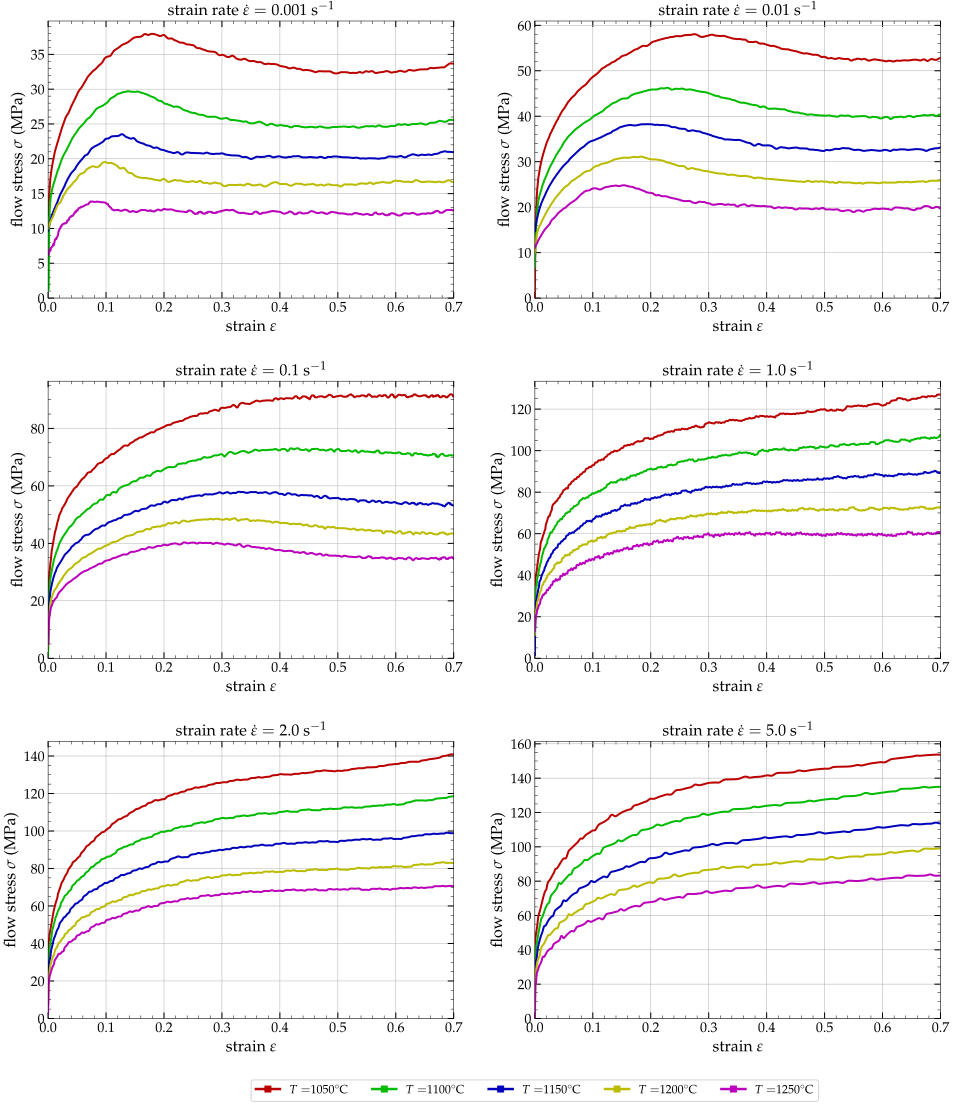
\includegraphics[width=0.9\columnwidth]{Figures/rawData}
\caption{Stress--strain curves of medium carbon alloy extracted from the Gleeble device for 5 temperatures ($T$) and 6 strain rates ($\mdot\varepsilon$).}
\label{fig:RawData}
\end{figure}

The flow stress ($\sigma$) increases with increasing strain rate ($\mdot\varepsilon$) but decreases with increasing temperature ($T$).
It is noteworthy that the flow stress is also influenced by the strain.
For the lowest strain rates, the flow stress increases up-to $\sigma_p$ with the strain until reaching a value of approximately $\varepsilon_p=0.2$ to $0.3$.
Subsequently, it decreases to maintain a relatively constant value throughout the test.
Conversely, for the highest strain rates (above $1~\ps$), the flow stress consistently increases during the entire test duration.
The slight increase in stress at low strain rates with large strain values is due to friction between the sample and the anvil during testing as reported by Galos \eal \cite{Galos-2022}.
This frictional effect becomes more pronounced as lubrication decreases over time.

The initial stress increase observed during deformation up to $\varepsilon=0.1$ is attributed to work hardening (WH).
Subsequently, from $\varepsilon=0.1$ to $0.2$, the flow stress demonstrates a continuous decline as the stress level increases until a peak or inflection point is reached, indicating the dominant influence of thermal softening surpassing work hardening.
At this stage, the stress-strain curve exhibits three different patterns as the strain increases: (i) gradual decrease to a steady state with DRV/DRX softening.
This pattern is observed for all deformation temperatures and strain rates ranging from $\mdot\varepsilon=0.001~\ps$ to $0.1~\ps$, except for those at $1050\celsius$ and $1100\celsius$; (ii) higher stress levels without significant softening and work hardening at $1050\celsius$ and $1100\celsius$ with a strain rate of $0.1~\ps$; (iii) continuous increase with significant work hardening observed for all deformation temperatures and a strain rate of $1~\ps$.
This suggests that softening due to DRX occurs at high temperatures and low strain rates.
In contrast, at higher strain rates and lower temperatures, the rate of softening due to DRX is slowed down by higher work hardening rates.
As a result, both the peak stress $\sigma_p$ and the onset of steady-state flow occur at higher strain levels.
The drop in stress observed at all temperatures and strain rates of $\mdot\varepsilon=0.001-5.0~\ps$ is due to the occurrence of DRX.

DRX is an important phenomenon for controlling the microstructural and mechanical properties of a material during hot working.
In some materials, such as aluminum, DRX can balance work hardening, resulting in the rapid appearance of a plateau.
However, in many austenitic steels, the kinetics of restoration are weak and, as a result, DRX can be triggered at a critical condition of strain accumulation.
Because of the significant influence of DRX on the material's flow stress at high temperature, this inevitably affects the material's microstructure after hot working, and prediction of the critical conditions for the onset of DRX is therefore crucial to good material characterization.
Several factors, such as the chemical composition of the material, the grain size before deformation, the mode of deformation and the deformation parameters (deformation rate, temperature and deformation) condition DRX, which can only be triggered if the critical deformation is reached, and this deformation can be determined using metallography.
However, this technique requires extensive sampling before and after critical deformation.
In addition, phase changes during cooling from the hot working temperature modify the deformed structure, making metallographic analysis difficult.
Hence the need for simpler techniques, such as the development of analytical models.
With this in mind, a number of studies have been carried out to determine analytically the initiation of DRX.

In this paper we will use the Johnson-Mehl-Avrami-Kohnogorov (JMAK) phenomenological model \cite{Avrami-1939} to compute the evolution of DRX of the material during the deformation.
The raw data acquired from the Gleeble thermosimulator will subsequently be used to identify the material flow law and the parameters of the DRX model.
The parameters of JMAK model are obtained through a two-step process.
Firstly, the critical stresses and strains are determined, where the ANN model is utilized to obtain well-filtered curves.
Secondly, these critical values are employed as input data for the calculation of parameters in the JMAK model, aiming to predict the volume fraction of dynamic recrystallization.

%----------------------------------------------------------------------------------
\subsection{DRX model's parameters identification\label{subsec:DRXParameters}}
%----------------------------------------------------------------------------------

In this Section we will determine the critical deformation required to initiate recrystallization.
Ryan and McQueen \cite{Ryan-1989, Ryan-1990, Ryan-1990-2} were the first to study this phenomenon, observing the appearance of an inflection point on the curve $\theta(\sigma)=\frac{\partial \sigma}{\partial \varepsilon}$ before the peak stress $\sigma_p$ and attributed to this inflection point the start of DRX and therefore the critical values $\varepsilon_c$ and $\sigma_c$ of the strain and the stress respectively.
Later Poliak and Jonas \cite{Poliak-1996, Poliak-2003, Poliak-2003-2, Jonas-2003} further demonstrated that this inflection point is associated with a thermodynamic free energy released during dislocation motion, and consequently endorse the DRX hypothesis describing this inflection point.
Najafizadeh and Jonas \cite{Najafizadeh-2006} simplified the thermodynamic model of Poliak and Jonas by developing an analytical technique, widely used today, to determine the critical conditions for the initiation of DRX.
In their approach, a polynomial of $3^\text{th}$ degree is adopted to describe the shape of the curve $\theta(\sigma)$ and, using the second derivative, they manage to identify the critical stress and strain ($\sigma_c$ and $\varepsilon_c$).

As introduced earlier, the determination of critical values for the initiation of DRX involves determining the inflection point located on the $\theta(\sigma)$ curve between $\varepsilon=0$ and $\varepsilon_c$.
One of the first difficulties is to numerically evaluate the value of the derivative of stress versus strain, since experimental data from compression tests show oscillations, as illustrated in Figure \ref{fig:RawData}.
It is therefore not possible to calculate the derivative $\theta(\sigma)=\frac{\partial \sigma}{\partial \varepsilon}$ directly.

To get around this problem, some authors recommend smoothing the experimental data (using the Excel solver for example \cite{Najafizadeh-2006}) or identifying an analytical form (e.g. a polynomial of relatively high order) using a minimization algorithm.
But, depending on the degree of the polynomial and for the same stress/strain curve, several solutions can be obtained, leading to the definition of several possible forms for the $\theta(\sigma)$ function.

%----------------------------------------------------------------------------------
\subsubsection{ANN based filtering model's archicture \label{subsec:ANNbasics}}
%----------------------------------------------------------------------------------
In order to improve the results obtained from the critical value identification procedure, we propose here to use the universal approximator capability of artificial neural networks to replace each strain-hardening curve by its representation in the form of an ANN with 1 input (strain) and 1 output (stress).
In such a network, each layer of neurons is connected to the one before it and the one after it by weighted connections.
Any hidden layer $k$, containing $n$ neurons, takes a weighted sum of the outputs $\overrightarrow{\hat{y}}$ of the immediately preceding layer $(k-1)$, containing $m$ neurons, given by the following~equation:
\begin{equation}
y_i\lay{k} = \sum_{j=1}^m w_{ij}\lay{k} \hat{y}_j^{(k-1)}+ b_i\lay{k},\label{eq:ANN1}
\end{equation}
where $y_i\lay{k}$ is the entry of the $i$th neuron of layer $k$, $\hat{y}_j\lay{k-1}$ is the output of the $j$th neuron of layer $(k-1)$, $w_{ij}\lay{k}$ is the associated weight parameter between the $i$th neuron of layer $k$ and the $j$th neuron of layer $(k-1)$, and $b_i\lay{k}$ is the associated bias of the $i$th neuron of layer $k$.
Those weights $w_{ij}$ and bias $b_i$, for each layer, are the training parameters of the ANN, which we have to adjust during the training procedure.
For the proposed model, we selected the Sigmoid activation function, so that each neuron in the hidden layer $k$ provides an output value ${\hat{y}}$ from the input value $y$ of the same neuron defined by Equation (\ref{eq:ANN1}) according to the following equation:
\begin{equation}
\hat{y}=\frac{1}{1 + \e{-y}}\label{eq:ANN2}
\end{equation}

No activation function was used for the output neuron of the ANN as usually done in a regression application.
The architecture chosen for our application corresponds to 2 hidden layers of 7 and 5 neurons respectively, as illustrated in Figure \ref{fig:ANN-7-5}.
If $n$ and $m$ are the number of neurons of the first and second hidden layers respectively, the number of internal parameters $N_{int}$ of the model is given by $N_{int}=m(2+n)+2n+1$.
So that for a $7-5$ network, $N_{int}=60$.
\begin{figure}[H]
%\centering
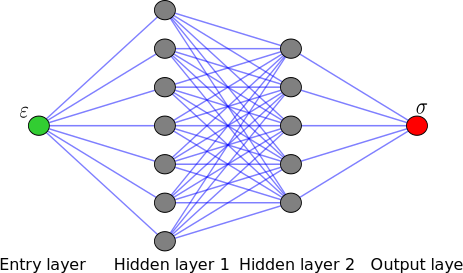
\includegraphics[width=0.7\columnwidth]{Figures/ANN-7-5}
\caption{Two hidden layers artificial neural network architecture with 1 input neuron (green) and 1 output neuron (red).}
\label{fig:ANN-7-5}
\end{figure}
The Python program used for training the neural network was developed using the specialized Python library, Tensorflow \cite{Abadi-2016}.
The Adaptive Moment Estimation (ADAM) optimizer \cite{Kingma-2015} was used for the training phase.

%----------------------------------------------------------------------------------
\subsubsection{ANN filtering based model's application \label{subsec:ANNapplication}}
%----------------------------------------------------------------------------------
Since the DRX occurs only for the 4 strain rates within the range $[0.001~\ps-1.0~\ps]$, we will only use the first 20 stress/strain curves for the DRX critical parameters' identification.
Each of the 20 curves, made up of 701 couples of strain-stress values, was processed independently by a neural network, leading to 20 identified architectures.
As an example, Figure \ref{fig:AnnFit} shows the experimental values of the stress/strain curve for $\mdot\varepsilon=0.001~\ps$ and $T=1050\celsius$ (blue line) and the results from the neural network identified from these data (red line).
\begin{figure}[H]
%\centering
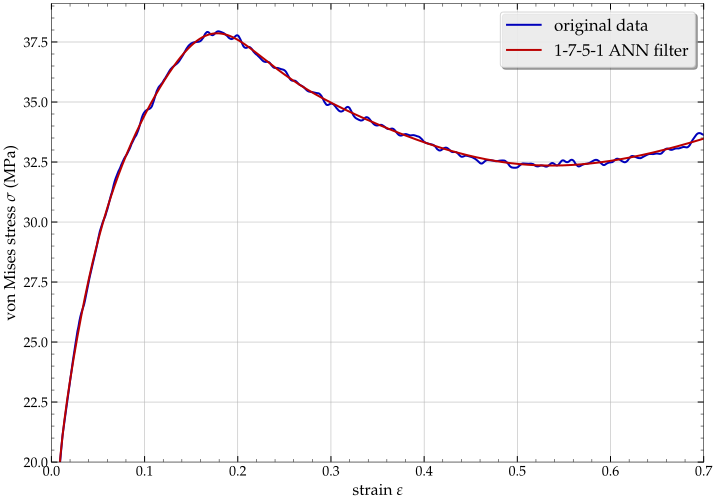
\includegraphics[width=0.7\columnwidth]{Figures/AnnFit}
\caption{Two hidden layers artificial neural network architecture with 1 input neuron (green) and 1 output neuron (red).}
\label{fig:AnnFit}
\end{figure}
The accuracy and predictive ability of the models are usually assessed through certain coefficients such as the mean absolute relative error ($\MARE$) defined by Equation (\ref{eq:AARE}):
\begin{equation}
\MARE(\%) = \frac{1}{N} \sum_{i=1}^{N}{\left|\frac{\sigma_i^p -\sigma_i^e}{\sigma_i^e}\right|} \times 100, \label{eq:AARE}
\end{equation}
and the root-mean-squared error ($\RMSE$) defined by Equation (\ref{eq:RMSE}):
\begin{equation}
\RMSE (\MPa) = \sqrt{\frac{1}{N} \sum_{i=1}^{N} \left(\sigma_i^p - \sigma_i^e\right)^2}, \label{eq:RMSE}
\end{equation}
where $\sigma_i^e$ is the experimental value, $\sigma_i^p$ is the value of the stress $\sigma$ predicted using the given model, and $N$ is the total number of data points used to compute those coefficients.
For the proposed ANN filter $\RMSE=0.093~\MPa$ and $\MARE=0.231~\%$, while using a $11^{th}$ order polynomial fit of the experimental data leads to $\RMSE=0.120~\MPa$ and $\MARE=0.275~\%$.

It can clearly be observed that using the ANN model to describe the $\sigma=f(\varepsilon)$ curve is better than using a $11^{th}$ order polynomial fit, as evidenced by the lower estimated error.
Therefore, this architecture of the ANN model is employed for the remaining curves, leading directly to deduce the hardening $\theta=f(\sigma)$ curves, which represent the rate of change of stress with respect to strain ($\frac{\partial \sigma}{\partial \varepsilon}$).
An example of computing the hardening curve for one temperature is given on Figure \ref{fig:AnnTheta} and for remaining temperatures, Figure \ref{fig:nThetaOP} can give an overview.
The same procedure is used for the four initial strain rates.
These curves provide essential information about critical stresses and strains needed for predicting DRX in the subsequent analysis.

\begin{figure}[H]
%\centering
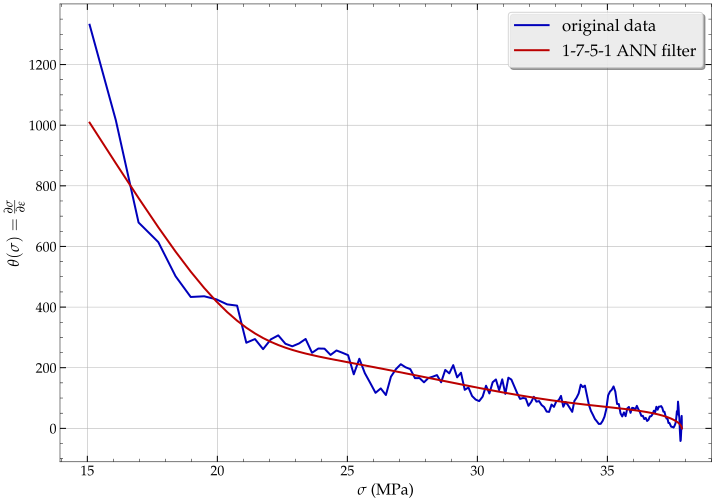
\includegraphics[width=0.7\columnwidth]{Figures/AnnTheta}
\caption{An example of computing hardening curve based on ANN model.}
\label{fig:AnnTheta}
\end{figure}

\begin{figure}[H]
%\centering
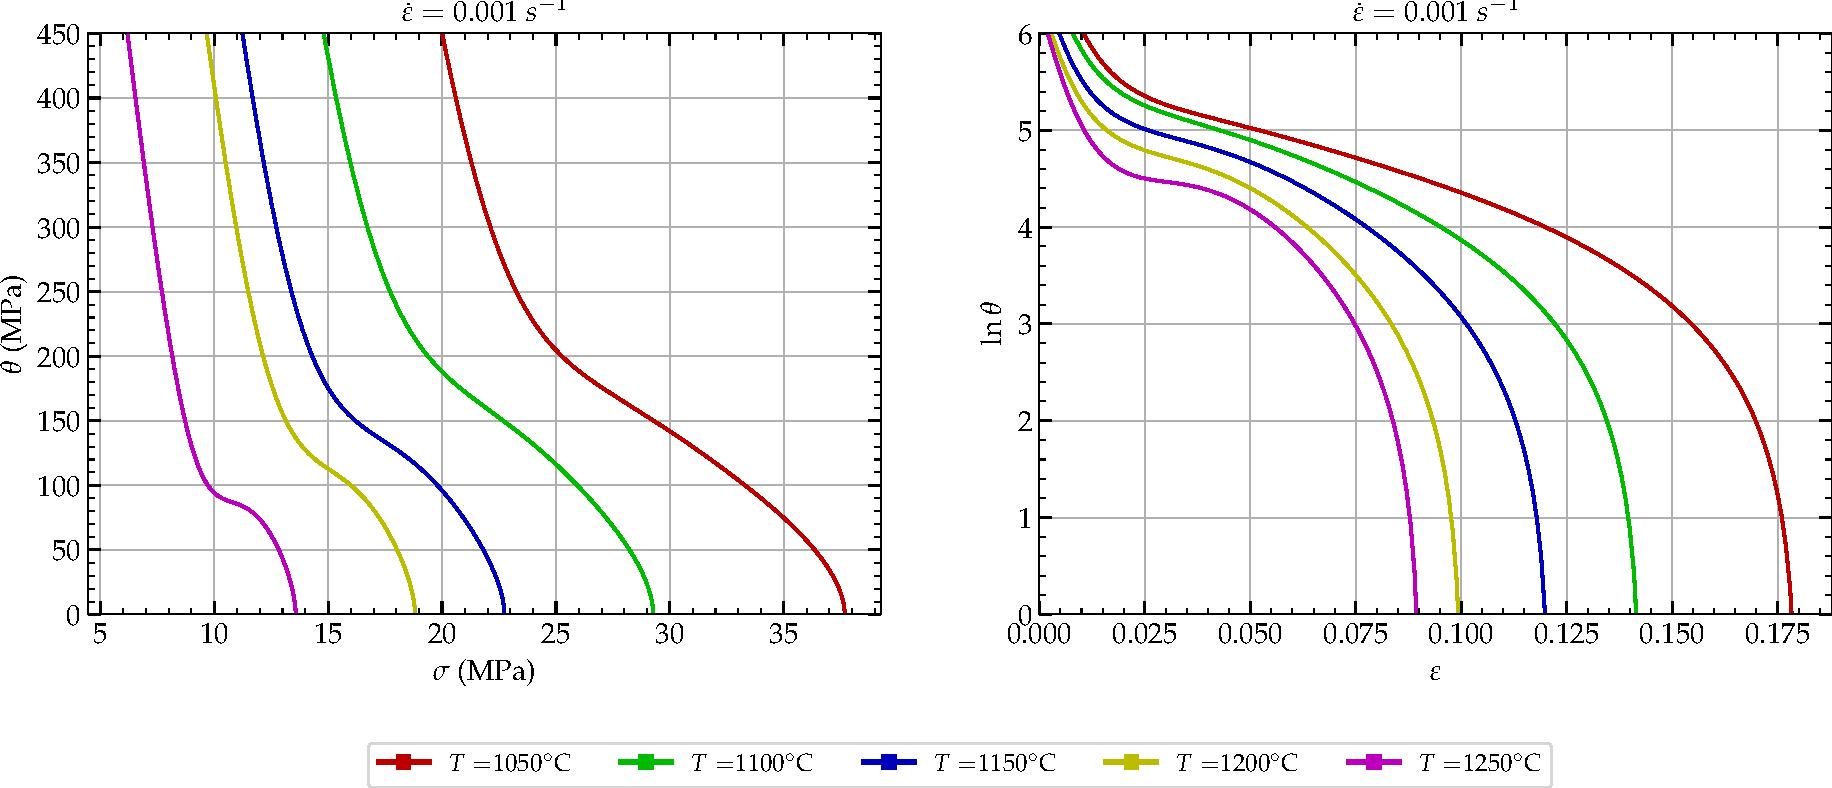
\includegraphics[width=0.99\columnwidth]{Figures/nThetaOP}
\caption{Work hardening computation for $1$ strain rate and $5$ temperatures.}
\label{fig:nThetaOP}
\end{figure}

%----------------------------------------------------------------------------------
\subsubsection{Critical conditions evaluation\label{subsec:CrConditions}}
%----------------------------------------------------------------------------------
As mentioned in the previous section, dynamic recrystallization initiates if and only if a certain critical condition level is reached.
Determining these critical conditions remains challenging, as it requires the development of models capable of calculating the corresponding critical stress and strain.
Thus, the Poliak and Jonas \cite{Poliak-1996,ei2003initiation,ei2003critical,jonas2003critical} method, widely recognized today, will be employed in this study.
The method involves using a third-degree polynomial function to describe the functions $\theta(\sigma)$ and $\ln \theta(\varepsilon)$curves as shown in Figure \ref{fig:fThetaOP} , with the purpose of identifying the inflection points corresponding to critical stress $\sigma_c$ and critical strain $\varepsilon_c$.
Also from those curves, peak stress $\sigma_p$ and peak strain $\varepsilon_p$ can be deduced.
The Poliak and Jonas model \cite{Poliak-1996,ei2003initiation,ei2003critical,jonas2003critical} is given as follow:
\begin{equation}
\theta = A\sigma^3 + B\sigma^2 + C\sigma + D
\end{equation}
Where $A, B, C,$ and $D$ are constants specific to a given deformation condition.
The inflection point of a function is determined by setting the second derivative of that function to zero and the following equation is obtained:
\begin{equation}
\frac{d^2 \theta}{d \sigma^2} = 6A\sigma + 2B
\end{equation}
Therefore, the critical stress for the initiation of DRX is obtained as follows:
\begin{equation}
6A\sigma_c + 2B = 0 \Longrightarrow \sigma_c = -B/3A
\end{equation}
Similarly, the critical strain is calculated using the following equations:
\begin{equation}
\ln \theta = A_1\varepsilon^3 + B_1\varepsilon^2 + C_1\varepsilon + D_1
\end{equation}
\begin{equation}
\frac{d^2 \ln \theta}{d \varepsilon^2} = 6\varepsilon A_1 + 2B_1 ~~\text{and} ~~\frac{d^2 \ln \theta}{d \varepsilon^2}= 0 \Longrightarrow \varepsilon_c = -B_1/3A_1
\end{equation}
Applying the same method to the first four strain rates and all temperatures, the critical stress and strain, peak stress and peak strain are summarised in the Table \ref{tab:OPparams}.
Once the critical conditions of the DRX are known, therefore they can be used as input to deduce the volume fraction of the DRX, which will be the subject of the next section.
\begin{figure}[H]
%\centering
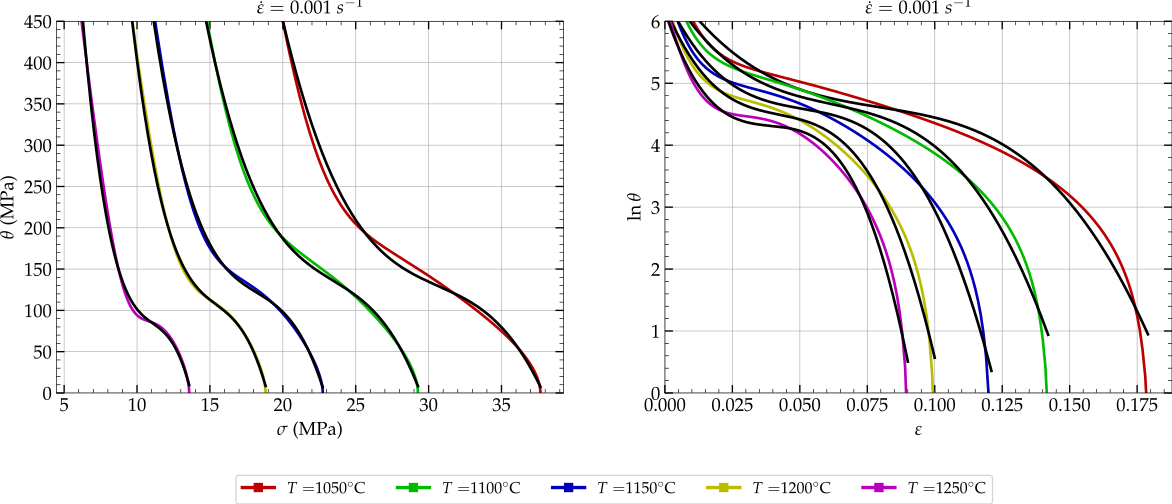
\includegraphics[width=0.99\columnwidth]{Figures/fThetaOP}
\caption{Work hardening polynomial fiting based on Poliak and Jonas model \cite{najafizadeh2006predicting}.}
\label{fig:fThetaOP}
\end{figure}


\begin{comment}
\begin{landscape}
\begin{table}[h]
\caption{functions $\theta=f(\sigma)$ and $\ln\theta=f(\varepsilon)$ coefficients based on Poliak and Jonas model \cite{najafizadeh2006predicting}.}\vspace{1mm}
%\begin{center}
\begin{tabular}{cccc}
\toprule
$\mdot{\varepsilon}~~(\text{s}^{-1})$ & $T$ ($^\circ$C) & $\theta$ = f($\sigma$) & $\ln$$\theta$=f($\varepsilon$)\\
\hline
&$1050	$&$ -0.252593\sigma^3 + 23.2834\sigma^2 - 719.045\sigma + 7561.2	 $&$-2274.82\varepsilon^3 + 592.899\varepsilon^2 - 61.0014\varepsilon + 6.71048$\\
&$1100	$&$ -0.469287\sigma^3 + 35.0169\sigma^2 - 875.042\sigma + 7418.89	 $&$-4813.49\varepsilon^3 + 1020.98\varepsilon^2 - 79.8778\varepsilon + 6.65741$\\
$0.001	$&$1150	$&$ -0.280343\sigma^3 + 15.2183\sigma^2 - 287.655\sigma + 2008.9	 $&$-899.654\varepsilon^3 + 15.7144\varepsilon^2 - 17.0976\varepsilon + 5.59789$\\
&$1200	$&$ -0.165122\sigma^3 + 7.34045\sigma^2 - 127.854\sigma + 949.691	 $&$10803.3\varepsilon^3 - 1567.6\varepsilon^2 + 31.5185\varepsilon + 4.92891$\\
&$1250	$&$ 0.430135\sigma^3 - 13.9807\sigma^2 + 123.725\sigma - 137.032 	 $&$-9130.5\varepsilon^3 + 1125.18\varepsilon^2 - 69.4152\varepsilon + 5.34578$\\
%\hline
&$1050	$&$ -0.316563\sigma^3 + 41.6041\sigma^2 - 1780.61\sigma + 24890.6	 $&$-760.548\varepsilon^3 + 302.444\varepsilon^2 - 47.4264\varepsilon + 6.96767$\\
&$1100	$&$-0.254362\sigma^3 + 27.7695\sigma^2 - 1002.47\sigma + 12089.1  $&$-957.925\varepsilon^3 + 326.362\varepsilon^2 - 48.1866\varepsilon + 6.78809$\\
$0.01	$&$1150	$&$ -0.125197\sigma^3 + 11.765\sigma^2 - 378.088\sigma + 4266.7$&$-1904.84\varepsilon^3 + 452.618\varepsilon^2 - 46.9027\varepsilon + 6.35515$\\
&$1200	$&$ -0.386264\sigma^3 + 28.6922\sigma^2 - 713.252\sigma + 6045.79	 $&$-1260.32\varepsilon^3 + 283.718\varepsilon^2 - 39.3944 \varepsilon + 6.12705$\\
&$1250	$&$ -0.274371\sigma^3 + 15.2491\sigma^2 - 291.928\sigma + 2051.22	 $&$2054.13\varepsilon^3 - 545.571\varepsilon^2 + 11.6535\varepsilon + 5.15417$\\
%\hline
&$1050	$&$ -0.109041\sigma^3 + 22.8574\sigma^2 - 1554.51\sigma + 34276.6	 $&$22.5257\varepsilon^3 - 10.6333\varepsilon^2 - 10.5919\varepsilon + 6.15546$\\
&$1100	$&$ -0.197437\sigma^3 + 32.5449\sigma^2 - 1740.23\sigma + 30179.2	 $&$-119.588\varepsilon^3 + 98.0419\varepsilon^2 - 32.5318\varepsilon + 6.75459$\\
$0.1	$&$1150	$&$ -0.273236\sigma^3 + 36.2143\sigma^2 - 1566.6\sigma + 22180.5	 $&$-245.608\varepsilon^3 + 155.747\varepsilon^2 - 40.2746\varepsilon + 6.76$\\
&$1200	$&$ -0.263314\sigma^3 + 29.6662\sigma^2 - 1095.93\sigma + 13363.4	 $&$-113.711\varepsilon^3 + 65.8505\varepsilon^2 - 25.9935\varepsilon + 6.30479$\\
&$1250	$&$ -0.390101\sigma^3 + 36.635\sigma^2 - 1132.85\sigma + 11626.3	 $&$-66.6657\varepsilon^3 + 88.2893\varepsilon^2 - 33.1747\varepsilon + 6.35758$\\
%\hline
&$1050	$&$ -0.0746046\sigma^3 + 21.1153\sigma^2 - 1933.09\sigma + 56923.3  $&$ -23.0014\varepsilon^3 + 42.4459\varepsilon^2 - 23.8994\varepsilon + 6.7553$\\
&$1100	$&$ -0.107164\sigma^3 + 25.6015\sigma^2 - 1978.33\sigma + 49199	 $&$-13.408\varepsilon^3 + 30.6189\varepsilon^2 - 20.0411\varepsilon + 6.3443$\\
$1	$&$1150	$&$ -0.139902\sigma^3 + 27.9237\sigma^2 - 1799.15\sigma + 37231	 $&$-14.1508\varepsilon^3 + 30.1129\varepsilon^2 - 19.4669\varepsilon + 6.11887$\\
&$1200	$&$ -0.150668\sigma^3 + 25.0242\sigma^2 - 1351.37\sigma + 23734.1	 $&$ 26.6437\varepsilon^3 - 11.2098\varepsilon^2 - 9.52699\varepsilon + 5.39017$\\
&$1250	$&$ -0.112709\sigma^3 + 16.0385\sigma^2 - 751.823\sigma + 11702	 $&$ 55.0921\varepsilon^3 - 38.055\varepsilon^2 - 4.07206\varepsilon + 4.95987$\\
\bottomrule
\end{tabular}
%\end{center}
\label{tab:JJparams1}
\end{table}
\end{landscape}
\end{comment}

\begin{table}[h!]
%\centering
\caption{Critical conditions based on Poliak and Jonas model \cite{najafizadeh2006predicting}.}\vspace{-1mm}
\begin{tabular}{cccccc}
\toprule
$\mdot{\varepsilon}~~(\text{s}^{-1})$ & $T$ ($^\circ$C) & $\varepsilon_p$ & $\sigma_p$ (MPa)& $\varepsilon_c$ & $\sigma_c$ (MPa) \\
\hline
     & $1050$ & $0.178$ & $37.862$& $0.083$ & $33.050$ \\
& $1100$ & $0.143$ & $29.770$ & $0.067$ & $25.648$ \\
$0.001$ & $1150$ & $0.124$ & $23.330$& $0.051$ & $19.116$ \\
& $1200$ & $0.102$ & $19.373$ & $0.039$ & $16.244$ \\
& $1250$ & $0.084$ & $13.883$ & $0.035$ & $11.302$ \\

& $1050$ & $0.281$ & $57.915$ & $0.131$ & $51.602$ \\
& $1100$ & $0.228$ & $46.107$ & $0.108$ & $40.495$ \\
$0.01$  & $1150$ & $0.195$ & $38.249$& $0.086$ & $33.435$ \\
& $1200$ & $0.172$ & $30.991$ & $0.076$ & $26.718$ \\
& $1250$ & $0.139$ & $24.739$ & $0.051$ & $20.004$ \\

& $1050$ & $0.571$ & $91.413$ & $0.244$ & $83.814$ \\
& $1100$ & $0.430$ & $72.662$ & $0.194$ & $65.259$ \\
$0.1$  & $1150$ & $0.344$ & $57.774$& $0.160$ & $51.723$ \\
& $1200$ & $0.299$ & $48.473$ & $0.136$ & $42.386$ \\
& $1250$ & $0.259$ & $40.195$ & $0.119$ & $35.277$ \\

& $1050$ & $0.700$ & $127.172$&$0.577$ &$116.1$ \\
& $1100$ & $0.700$ & $106.608$& $0.329$ & $94.51$ \\
$1$   & $1150$ & $0.700$ & $89.525$& $0.268$ & $89.067$ \\
& $1200$ & $0.700$ & $72.270$ & $0.178$ & $57.929$ \\
& $1250$ & $0.393$ & $59.992$ & $0.112$ & $54.066$ \\
\bottomrule
\end{tabular}
\label{tab:OPparams}
\end{table}

%----------------------------------------------------------------------------------
\subsection{DRX model parameters evaluation\label{subsec:DRXparams}}
%----------------------------------------------------------------------------------
The DRX begins at a critical deformation, as previously mentioned, and the level of recrystallization can be determined experimentally.
Figure \ref{fig:DRXschema} illustrates three stages of recrystallization: nucleation, grain growth, and grain coalescence.
\begin{figure}[!ht]
%\centering
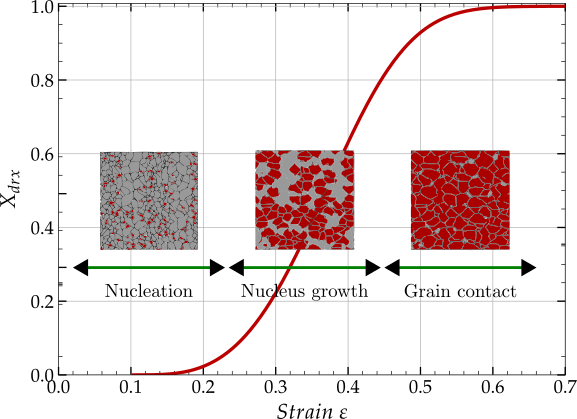
\includegraphics[width=0.7\columnwidth]{Figures/picDRX}
\caption[Diagramme des trois étapes de la DRX]{Diagramme des trois étapes de la DRX \cite{wan2017experimental}}
\label{fig:DRXschema}
\end{figure}
The subsequent behavior of DRX affects the material's flow stress curve as the rate of work hardening is influenced by dislocations within the free grains.
The Avrami model is the most commonly used law to predict this behavior, known as the JMAK model, whose expression is given by the following equation estimating the volumic fraction of the DRX:
\begin{equation}
X_{drx,pred} = 1 - \exp\left[ -k\left(\frac{\varepsilon - \varepsilon_c}{\varepsilon_p}\right)^{n_k}\right]
\label{eq:drxpred}
\end{equation}
With $\varepsilon_c$ and $\varepsilon_p$ as the critical and peak strain respectively; $k$ and $n_k$ as the model's parameters and the experimental equivalence of this volumic fraction of DRX is given by :
\begin{equation}
X_{drx,exp} = \frac{\sigma_p-\sigma}{\sigma_p-\sigma_{s}}
\label{eq:drxexp}
\end{equation}

Where $\sigma_p$ and $\sigma_s$ are the peak stress and the steady stress after the peak stress resectivly.
It is possible to establish a dependency relationship between these specific stresses/strains and the Zener-Hollomon parameter $Z = \mdot\varepsilon \exp{\left(\frac{Q}{RT}\right)} \label{eq:ArZ}$, according to the following equation:
\begin{equation}
\begin{cases}
\varepsilon_c = A_cZ^{n_c} \\ \varepsilon_p = A_pZ^{n_p} \\ \sigma_c = B_cZ^{m_c} \\ \sigma_p = B_pZ^{m_p}\\ \sigma_s = B_sZ^{m_s}
\end{cases}
\label{eq:paramsZ}
\end{equation}
With $A_{c,p}, n_{c,p}, B_{c,p,s}$ and $m_{c,p,s}$ the parameters describing the dependency of specific strains and stresses on the Zener-Hollomon parameter where their identification procedure is explained later in this paper.

The calculation of the parameters of JMAK model involves two main steps.
Firstly, it entails determining the coefficients $A_{c,p}, n_{c,p}, B_{c,p,s}$ and $m_{c,p,s}$.
Secondly, these coefficients are then incorporated into equation (\ref{eq:paramsZ}) for their final use in equations (\ref{eq:drxpred}) and (\ref{eq:drxexp}).
To compute these parameters, a Python code using the $curve\_fitting$ method is used.
Specifically, the critical strains and stresses calculated in the previous sections are used as input data for these parameter identifications.
The curve fitting method aims to find the best-fitting values for the coefficients by iteratively adjusting them to minimize the difference between the predicted and experimental critical strains and stresses.
This optimization process involves trying various combinations of the coefficients and evaluating their fitness to the given data.
The curve fitting technique adjusts the coefficients until it achieves the closest match between the model's predictions and the experimental values.


Once the constants that define the Zener-Hollomon parameter dependency are calculated, they can be used to deduce the JMAK model parameters using an optimization technique that minimizes the error between the predicted recrystallization $X_{drx, pred}$ and the experimental value $X_{drx, exp}$.
The dependency of the Zener-Hollomon parameters and the JMAK model parameters are provided in the Table \ref{tab:allparams}.

\begin{table}[h]
%\centering{}
\caption{JMAK model and Zener-Hollomon dependency parameters }\vspace{-1mm}
\begin{tabular}{cccccc}
\toprule
$A_c$ & $A_p$& $B_c$& $B_p$& $B_s$& $n_c$ \\
\hline
$4.4268\times10^{-5}$& $29.85\times10^{-5}$& $0.0720627$&$0.103141	$&$10265.8	$&$0.235832	$\\
\toprule
$n_p$ & $m_c$& $m_p$& $m_s$& $k$& $n_k$ \\
\hline
$0.203678	$& $0.188236$&$0.181822$&$-0.19708$&$0.48632$&$3.36531$\\
\bottomrule
\end{tabular}
\label{tab:allparams}
\end{table}


The curves of $X_{drx}(\varepsilon)$ are provided in Figure \ref{fig:nDRX} using the critical conditions calculated by the Poliak method.
From this figure, we can observe that the predictions align well with the experimental data, thus demonstrating the validity of the utilized model.
Therefore, these results will be used subsequently in the simulation section.
\begin{figure}[H]
\centering
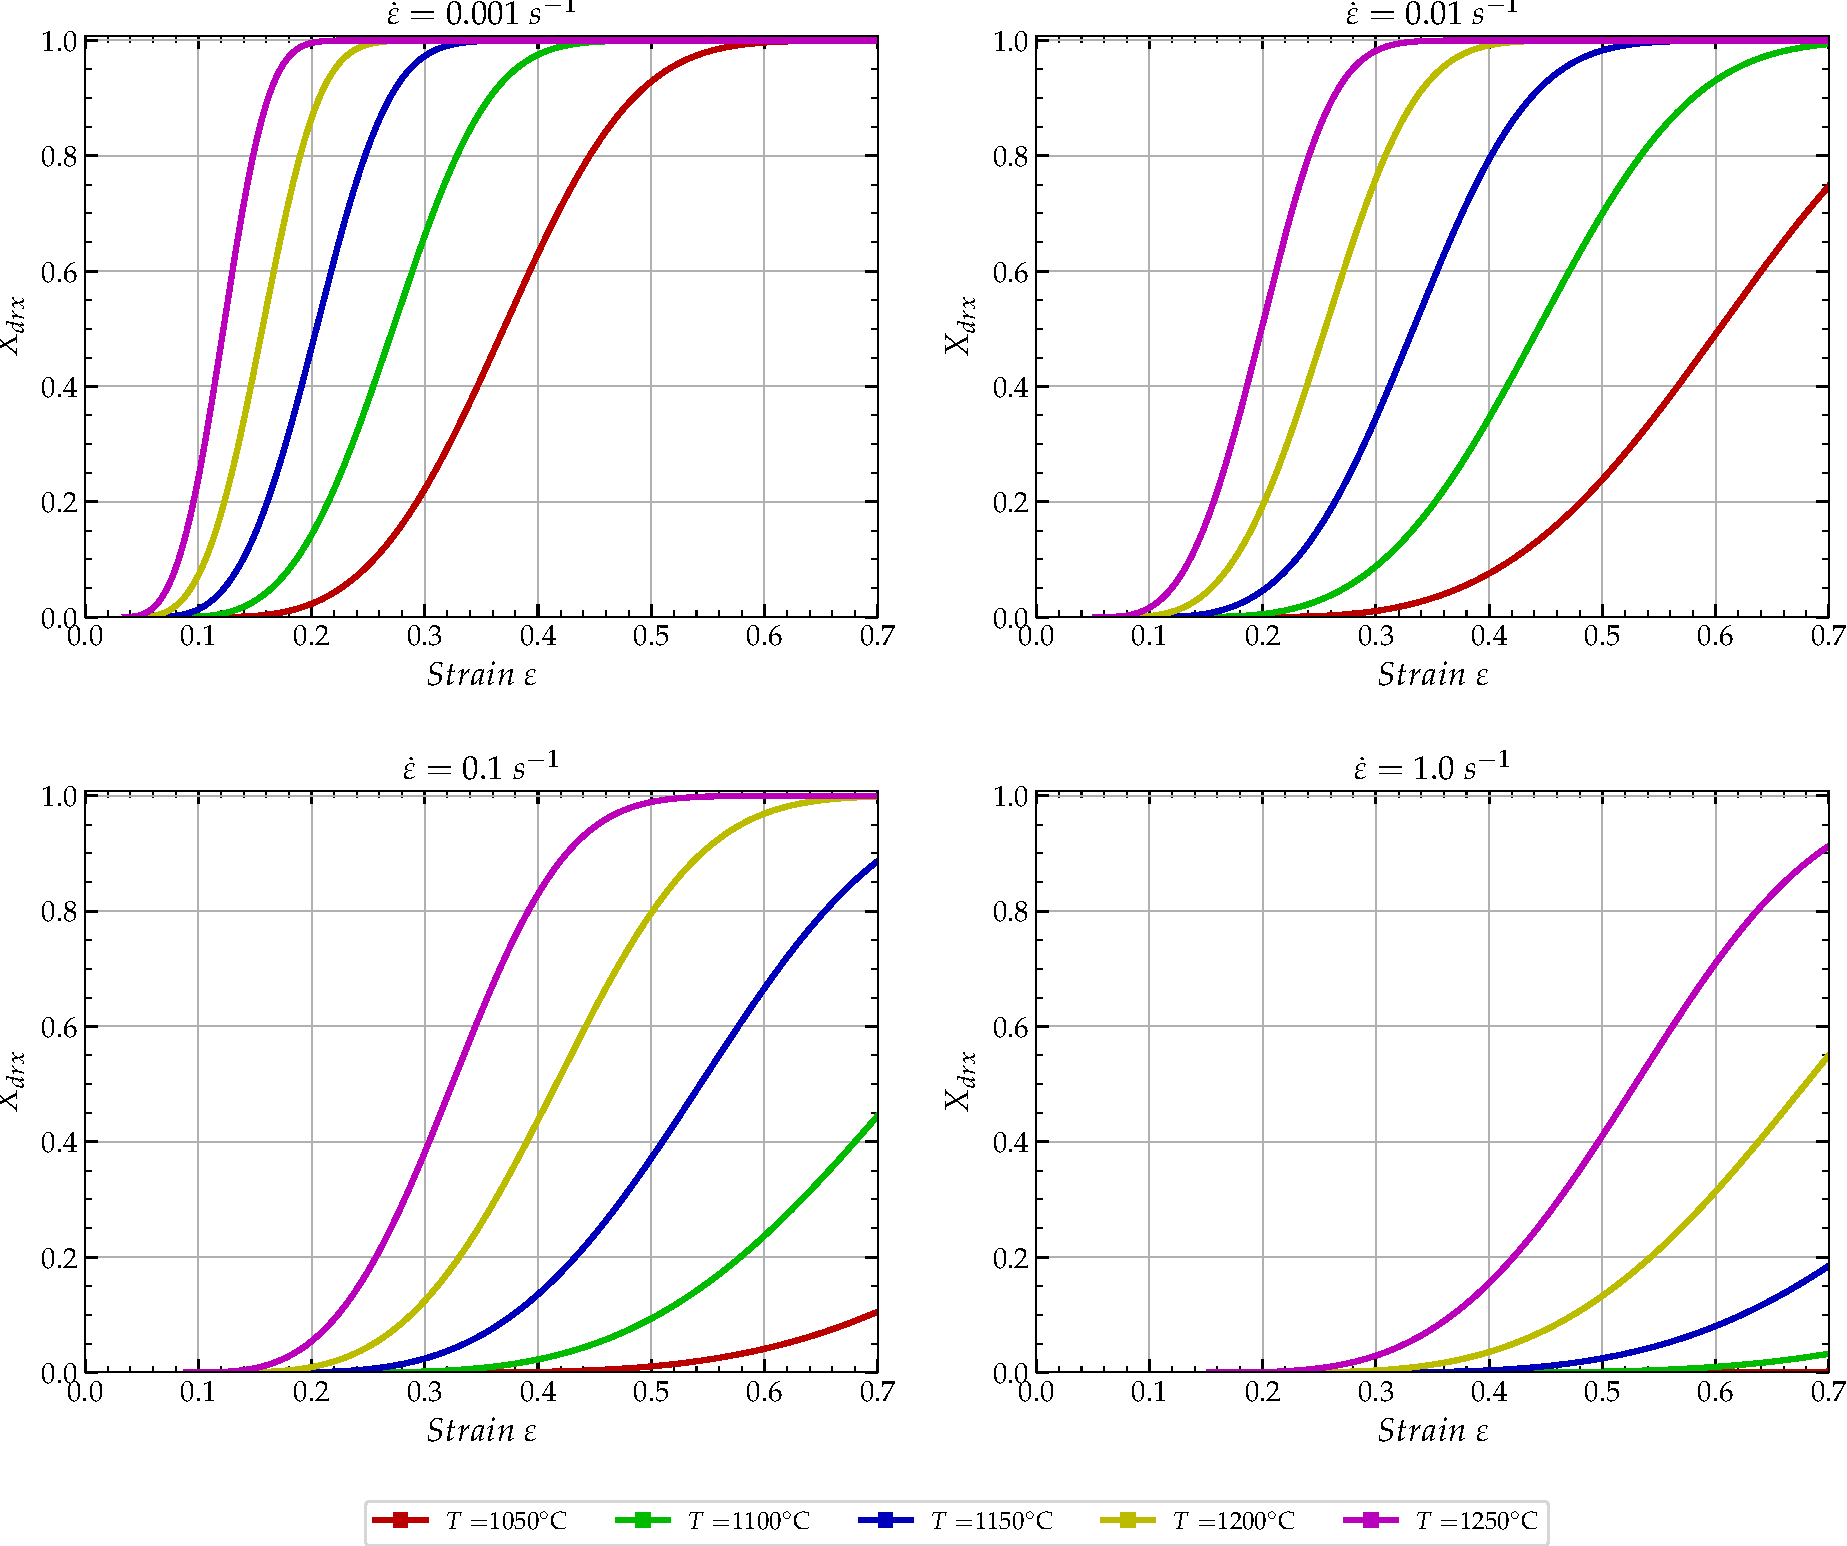
\includegraphics[width=0.99\columnwidth]{Figures/nDRX}
\caption{Comparision beteween DRX experimental data and JMAK model based prediction}
\label{fig:nDRX}
\end{figure}
%\begin{table}[H]
%\caption{Architecture and accuracy coefficients for all the proposed networks.}
%\newcolumntype{C}{>{\centering\arraybackslash}X}
%\newcolumntype{L}{>{\raggedright\arraybackslash}X}
%\begin{tabularx}{\textwidth}{LCCCCCC}
%\hline
%Coefficient & $\mdot\varepsilon$ & $1050\celsius$ & $1100\celsius$ & $1150\celsius$ & $1200\celsius$ & $1250\celsius$ \\
%\hline
%$\MARE(\%)$ & $0.001$ & $0.231$ & $1.13$ & $1.05$ & $1.08$ & $0.75$ \\
%$\RMSE(\MPa)$ & $0.001$ & $0.093$ & $0.59$ & $0.57$ & $0.65$ & $0.46$ \\
%\hline
%\end{tabularx}
%\label{tab:Errors}
%\end{table}

%----------------------------------------------------------------------------------
\section{Numerical simulation of the compression\label{sec:NumSim}}
%----------------------------------------------------------------------------------
In this section, the numerical validation of the previously performed dynamic recrystallization identification will be addressed.
To achieve this, it is essential to establish a constitutive law capable of accurately predicting the plastic deformation of the material.
In our prior publication (Tize Mha \eal \cite{TizeMha-2023}), a comparison between analytical constitutive laws and neural network based approache was conducted, resulting in the identification of an ANN model as the suitable choice for this material.
As a result, this section comprises a two-fold focus: firstly, a recapitulation of the ANN based constitutive law identification, as presented in the previous article; and secondly, the integration of this identified ANN model with the JMAK model for predicting dynamic recrystallization behaviour.
%----------------------------------------------------------------------------------
\subsection{Identification of the ANN constitutive law\label{subsec:ANNConstitutiveLaw}}
%----------------------------------------------------------------------------------
In general terms, flow stress $\sigma$ is a non-linear function of the strain $\varepsilon$, increasing with the strain rate $\mdot\varepsilon$, but decreasing with increasing temperature $T$.
The model can therefore be described as an elastoplastic model with the influence of strain rate and temperature.
This type of behavior generally leads to Johnson-Cook \cite{Johnson-1983}, Zerilli Armstrong \cite{Zerilli-1987}, Hansel Spittle \cite{Hensel-1978} or Arrhenius \cite{Sellars-1966} flow law type.
Depending on the nature of the stress-strain relationship, modeling with one or other of these models can take into account the actual behavior of the material at certain strain rates.
As reported by Tize Mha \eal \cite{TizeMha-2023}, Johnson-Cook, Zerilli Armstrong or Hansel Spittle type models, while providing a more or less faithful reproduction of material behavior at strain rates above $1~\ps$, do not take into account the softening due to DRX visible on experimental curves for strain rates below $1~\ps$ as reported in Figure \ref{fig:RawData}.
Indeed, for the lowest strain rates, the flow stress $\sigma$ increases with strain $\varepsilon$ up to a value of around $\varepsilon=0.2$ to $0.3$ and then decreases to maintain a more or less constant value until the end of the test.
Only the Arrhenius model can more or less account for this softening at low strain rates.
As proposed by Pantalé \eal \cite{Pantale-2021, Pantale-2023} and Tize Mha \eal \cite{TizeMha-2023}, an effective alternative is to use a flow law defined by an artificial neural network trained directly on experimental data from compression tests.
Correctly defining the hyperparameters of this neural network (number of hidden layers, number of neurons, activation functions, etc.) allows us to obtain a flow law that faithfully reproduces the data obtained from compression tests.

According to the method proposed by Pantalé \eal \cite{Pantale-2021, Pantale-2023}, we developed in Tize Mha \eal \cite{TizeMha-2023} a two hidden layers ANN based flow law whose general structure is reported in Figure \ref{fig:ANN-2HL}.
This ANN contains an input layer of three neurons corresponding to the entries of the model ($\varepsilon$, $\mdot\varepsilon$ and $T$), an output layer with one neuron ($\sigma$), and $2$ hidden layers.

All details about the artificial neural network, setup of the experimental data and the training method is reported the paper proposed by Pantalé \cite{Pantale-2023}.
%Thus, all the neurons of the $k^{th}$ layer are connected to all the neurons of the ($k-1^{th}$) layer, as shown in~Figure~\ref{fig:ANN-2HL}.

\begin{figure}[H]
%\centering
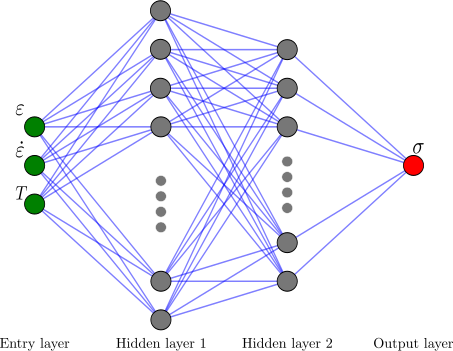
\includegraphics[width=0.55\columnwidth]{Figures/ANN-scheme-2HL}
\caption{Two hidden layers artificial neural network architecture with 3 inputs neurons (green) and 1 output neuron (red).}
\label{fig:ANN-2HL}
\end{figure}

We again used the Tensorflow library for the development of the training program, and the ADAM optimizer was used for the training phase.
The provided database presented in Section \ref{subsec:ExperimentalProcedure} consists of $21,030$ quadruplets of strain ($\varepsilon$), strain rate ($\mdot\varepsilon$), temperature ($T$) and stress ($\sigma$) values.
%The training data were those from the tests presented in Section \ref{sec:ComTestResults} and were composed of $21,030$ quadruplets of ($\varepsilon$, $\mdot\varepsilon$, $T$, $\sigma$) values.

We selected 6 different networks, named 3-$n$-$m$-1, where $n$ is the number of neurons in the first hidden layer and $m$ is the number of neurons in the second hidden layer, to show the importance of selecting the adequate number of neurons in the two layers.

The training was performed on the basis of $5000$ epochs of the experimental dataset.
It took $40$~min of training on a Dell XPS-13 7390 laptop running Ubuntu 22.04 LTS 64 bits with 16 GB of RAM and an Intel 4-core i7-10510U processor to obtain the converged parameters of the ANN model.

Figure \ref{fig:ANN-conv} shows the evolution of the training error defined by the $\log_{10}$ of the internal $\RMSE$ during the training phase and Table \ref{tab:Errors} summarizes the final values of this criterion, along with the final values of the $\MARE$ and the $\RMSE$ for the 6 configurations of the neural network.
On the basis of those results, we have selected the 3-15-7-1 network for further study, as it has the best convergence evolution and the lowest final error values ($\MARE=0.62\%$ and $\RMSE=0.38~\MPa$), while keeping a reasonable number of internal parameters ($N_{int}=180$).

\begin{figure}[H]
\centering
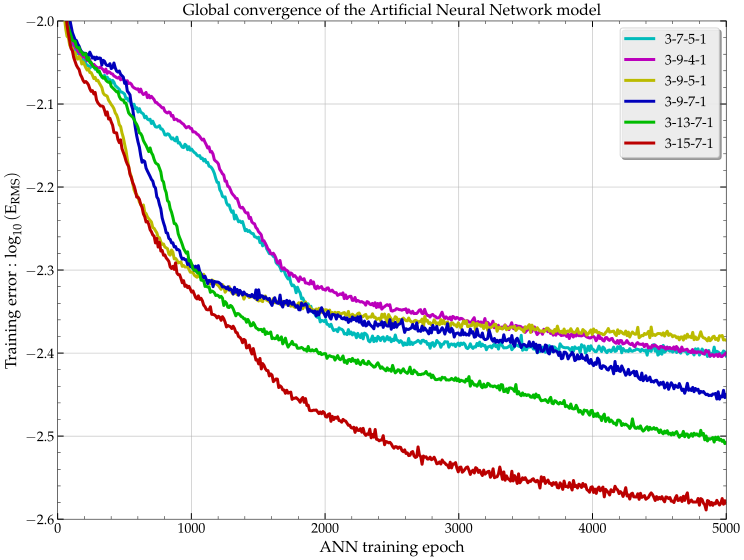
\includegraphics[width=0.7\columnwidth]{Figures/Conv-ANN-6}
\caption{Evolution of the convergence of the models during the training procedure for the 6 proposed network architectures.}
\label{fig:ANN-conv}
\end{figure}

\begin{table}[H]
\caption{Architecture and accuracy coefficients for all the proposed networks.}
\newcolumntype{C}{>{\centering\arraybackslash}X}
\newcolumntype{L}{>{\raggedright\arraybackslash}X}
\begin{tabularx}{\textwidth}{LCCCCCC}
\toprule
\textbf{Coefficients} & \textbf{3-7-5-1} & \textbf{3-9-4-1} & \textbf{3-9-5-1} & \textbf{3-9-7-1} & \textbf{3-13-7-1} & \textbf{3-15-7-1} \\
\hline
$N_{int}$ & $74$ & $81$ & $92$ & $114$ & $158$ &$180$\\
\toprule
$\log_{10}(\RMSE)$ & $-2.40$ & $-2.42$ & $-2.38$ & $-2.45$ & $-2.50$ & $-2.58$ \\
$\MARE(\%)$ & $1.13$ & $1.05$ & $1.08$ & $0.91$ & $0.75$ & $0.62$ \\
$\RMSE(\MPa)$ & $0.59$ & $0.57$ & $0.65$ & $0.55$ & $0.46$ & $0.38$ \\
\bottomrule
\end{tabularx}
\label{tab:Errors}
\end{table}

\begin{figure}[H]
\centering
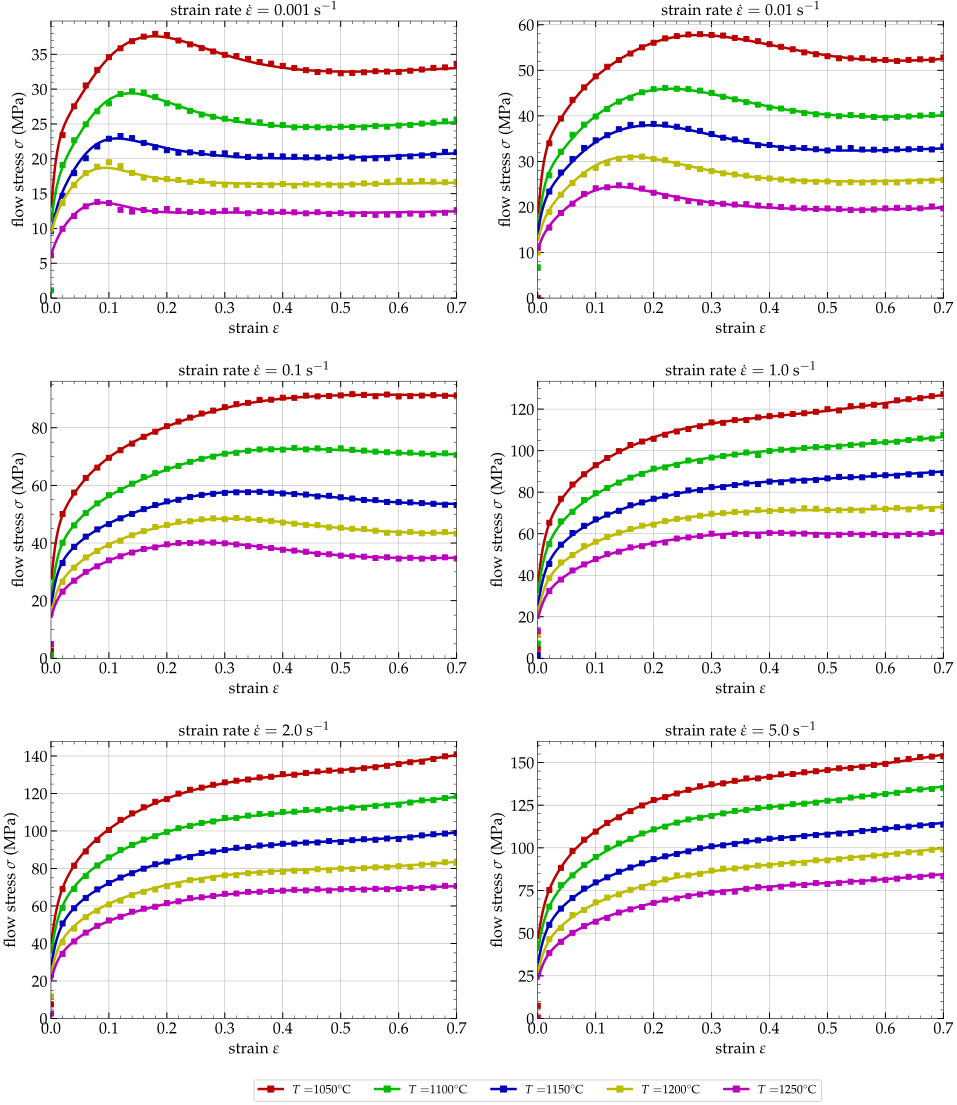
\includegraphics[width=0.9\columnwidth]{Figures/CompExpANN-3-15-7-1}
\caption{Comparison between the experimental (dots) and predicted (lines) flow stresses $\sigma$ by the 3-15-7-1 ANN model.}
\label{fig:ANN-3-15-7-1}
\end{figure}
This model will be used as the material flow law for the numerical simulations presented in Section \ref{subsec:DRXSimulation}.

%----------------------------------------------------------------------------------
\subsection{Dynamic recrystallization simulation\label{subsec:DRXSimulation}}
%----------------------------------------------------------------------------------
In order to assess the effectiveness of the implementation of the DRX model presented in the previous sections, a compression test is simulated in this section.
For this purpose, the material used for this simulation is a medium-carbon P20 iron alloy, which was used for the identification of this model.
An axisymmetric Finite Element Method (FEM) model of hot cylinder compression with a height of $15$ mm and a diameter of $5$ mm is used, as shown in Figure \ref{fig:Mesh}.
The frictional coefficient at the material/Die interface was assumed to be $0.2$ \cite{zhang2019elevated,sun2020kinetique}.
The mesh consists of 986 CAX4R elements (4-node axisymmetric bi-linear quadrilateral elements with reduced integration and hourglass control).
The FEM model is simulated using Abaqus/Implicit due to the computation time related to the low strain rates.
A displacement of $60\%, ~45\%, ~30\%$ and $15\%$ mm of the total height is imposed on the upper part of the cylinder during the compression along the vertical axis of the specimen.
The radial displacement $u_r$ of the upper part of the specimen is left free, while its axial displacement $u_z$ is imposed.
The lower part of the cylinder remains fixed during the simulation.
The effect of reducing the cylinder in combination with strain rate and temperature effect has been also evaluated in this simulation, and conclusions have been drawn.
For this simulation, three temperatures ($1050^\circ$C, $1150^\circ$C, and $1250^\circ$C) and four strain rates ($0.001~\text{s}^{-1}$, $0.01~\text{s}^{-1}$, $0.1~\text{s}^{-1}$ and $1.0~\text{s}^{-1}$) are considered.
\begin{figure}[H]
%\centering
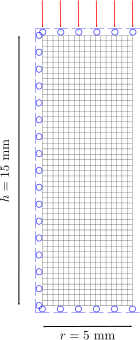
\includegraphics[width=0.6\columnwidth]{Figures/CyCompression2}
\caption{Numerical model for the compression test}
\label{fig:Mesh}
\end{figure}

%----------------------------------------------------------------------------------
\subsubsection{Temperature and strain rate effects \label{subsec:TempSReffect}}
%----------------------------------------------------------------------------------

Temperature and strain rate play a crucial role in influencing dynamic recrystallization in materials, particularly for metals and alloys in the sense that they lead to the formation of new grains within the material.
Indeed, higher temperature and low strain rate generally lead to increased nucleation rates and faster growth rates of new grains during dynamic recrystallization while in opposite lower temperature and higher strain rate lead to imcomplete dynamic recrystallization.
At elevated temperatures, the mobility of atoms and dislocations is enhanced, allowing for the creation of new grain boundaries and the growth of new grains.
This results in a finer and more equiaxed grain structure.
Also, higher temperatures can lead to a higher fraction of recrystallized material because the enhanced mobility of dislocations promotes the formation of new grains.
This can result in a significant change in the microstructure and mechanical properties of the material.
Figure \ref{fig:TempEffect} and Figure \ref{fig:SREffect} illustrate the simulated results of the DRX fraction of P20 steel under varying deformation conditions.
Figure \ref{fig:TempEffect} illustrates that as the temperature rises, the scope of dynamic recrystallization expands.
The gradual rise in the dynamic recrystallization fraction within the center is evident, spreading outward.
This expansion is attributed to heightened thermal activation and increased atomic diffusion at elevated temperatures, rendering the material more susceptible to dynamic recrystallization.
The $X_{drx}$ clearly increases with increasing temperature and reduction.
At $45\%$ and $60\%$ reduction, the $X_{drx}$ of P20 steel
reached $100\%$ in the central part of the specimen for all the initial sample temperatures.
Indeed, the plastic deformation of a material is accompanied by the creation of dislocations.
These dislocations represent a "store of elastic energy".
When the temperature is high enough, the dislocations become spontaneously mobile and cause a reorganisation of the crystal structure, in two stages: restoration and recrystallisation.
The nature of the phases does not change (those that are thermodynamically stable), the atoms keep the same lattice, but the grain boundaries and the orientation of the crystallites change.

\begin{figure}[H]
%\centering
\includegraphics[width=0.98\columnwidth]{Figures/Temp_DRX}
\caption{$X_{drx}$ values at a strain rate of $0.01~\text{s}^{-1}$ for different reductions and initial temperatures.}
\label{fig:TempEffect}
\end{figure}
\begin{figure}[H]
%\centering
\includegraphics[width=0.98\columnwidth]{Figures/SR_DRX}
\caption{$X_{drx}$ values at a fixed $T_0=1150^\circ$C for different reductions and strain rates.}
\label{fig:SREffect}
\end{figure}

The temperature at which these phenomena occur depends on the rate of deformation: the more a material is deformed, the more elastic energy it 'stores', so the earlier (at a lower temperature) restoration and recrystallisation will begin.
According to Figure \ref{fig:SREffect}, the magnitude of dynamic recrystallization diminishes with escalated strain rates, leading to a reduction in the extent of recrystallization.
This outcome is attributed to the accelerated pace of deformation at higher strain rates, elevating the critical strain and lowering the likelihood of internal dynamic recrystallization within the material.

%----------------------------------------------------------------------------------
\subsubsection{Experimental validation \label{subsec:ExpValid}}
%----------------------------------------------------------------------------------
In this section, a comparison beteween experimental and simulation will be carried out.
Indeed, the percentage of dynamic recrystallization of selected regions is observed and then compared to the simulation.
The Figure \ref{fig:expNumDRX} presents a comparison between experimental data and simulation for a test conducted at a temperature of $1150^\circ$C with a deformation strain rate $0.01~\text{s}^{-1}$.
Five zones have been selected to observe the percentage of recrystallization, which varies between $5\%$ and $100\%$.
In fact, $5\%$ corresponds to the value associated with the dead zone; which is the contact between the sample and die exposed to friction effects.
On the other hand, $100\%$ corresponds to the value observed at the center of the sample, where deformation is higher.
In the center of the sample, the temperature is high, leading to a significant accumulation of energy.
Conversely, at the edges of the sample, a relatively complete recrystallization is observed because the temperature during deformation migrates from the center towards the outer regions of the piece, enabling recrystallization to take place.
Microscopic observations corresponding to each zone reveal large grains (Figure \ref{fig:expNumDRX} (d)) in the dead zone, whereas small grains (Figure \ref{fig:expNumDRX} (a)) are observed at the center of the sample, resulting from complete recrystallization.
\begin{figure}[H]
%\centering
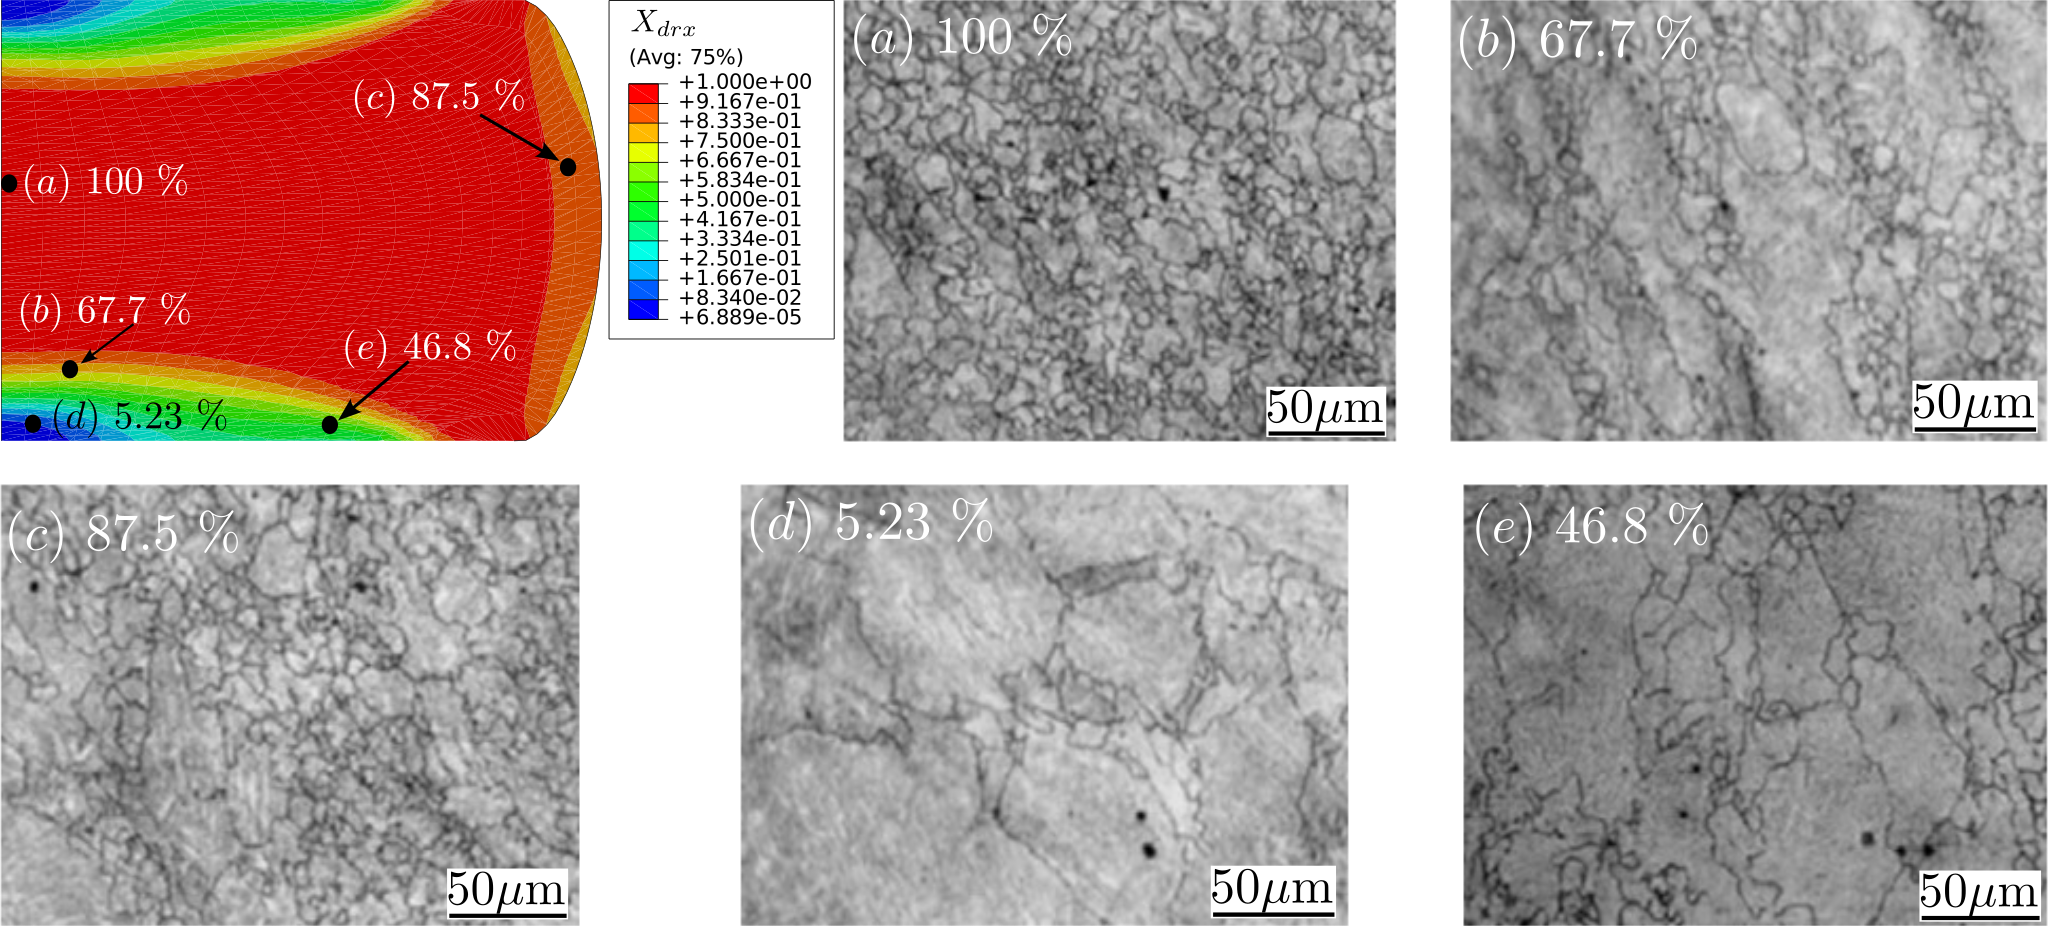
\includegraphics[width=0.98\columnwidth]{Figures/expNumDRX}
\caption{Experimental and numerical $X_{drx}$ values for $T_0=1150^\circ$C and strain rate $\mdot{\varepsilon}=0.01~\text{s}^{-1}$.}
\label{fig:expNumDRX}
\end{figure}
%----------------------------------------------------------------------------------
\section{Conclusions\label{sec:Conclusions}}
%----------------------------------------------------------------------------------
In this study, we have harnessed the capabilities of ANN technique to gain a profound understanding of the dynamic recrystallization process and its evolution under varying conditions.
The integration of ANN modeling, fundamental material models, simulation software, and experimental validation has led to a comprehensive framework that contributes significantly to the field of materials science and engineering.
Initially, we successfully employed a ANN model to fit flow stress curves, enabling the prediction of critical conditions using the Poliak model.
Doing this has allowed us to accurately anticipate the conditions at which the DRX process initiates, providing an invaluable tool for anticipating material behavior under specific deformation scenarios.

We harnessed the predicted critical conditions to feed into the JMAK model and by doing so, we achieved the prediction of the DRX volumic fraction, thereby offering insights into the kinetics and mechanisms governing recrystallization.
This integration bridges the gap between theoretical models and real-world phenomena, offering a deeper understanding of the intricate processes taking place during deformation.
Taking our investigation further, we have seamlessly integrated the JMAK model into the ABAQUS software, a widely-utilized platform for simulation and analysis.
Through this integration, we were able to simulate the evolution of DRX during hot compression tests, capturing the process's response to varying conditions.
By comparing our simulation results with experimental data and employing microstructure analysis, we validated the accuracy of our simulations and affirmed the efficacy of our predictive models.

It is important to note that while our research marks a significant milestone, it also presents opportunities for future exploration.
Fine-tuning our model, expanding our dataset, and refining the integration process can further enhance the accuracy and applicability of our predictions.
Moreover, the successful linkage of theory, simulation, and experimentation provides a robust framework for tackling complex material behavior challenges in industries spanning from manufacturing to aerospace.

%%%%%%%%%%%%%%%%%%%%%%%%%%%%%%%%%%%%%%%%%%
%\section{Patents}

%%%%%%%%%%%%%%%%%%%%%%%%%%%%%%%%%%%%%%%%%%
\vspace{6pt}

%%%%%%%%%%%%%%%%%%%%%%%%%%%%%%%%%%%%%%%%%%
%% optional
%\supplementary{The following supporting information can be downloaded at: \linksupplementary{s1}, Figure S1: title; Table S1: title; Video S1: title.}

% Only for the journal Methods and Protocols:
% If you wish to submit a video article, please do so with any other supplementary material.
% \supplementary{The following supporting information can be downloaded at: \linksupplementary{s1}, Figure S1: title; Table S1: title; Video S1: title. A supporting video article is available at doi: link.}

%%%%%%%%%%%%%%%%%%%%%%%%%%%%%%%%%%%%%%%%%%
\authorcontributions{
Conceptualization, P.T.M. and O.P.;
methodology, O.P.;
software, P.T.M. and O.P.;
validation, O.P.;
formal analysis, O.P.;
investigation, P.D.;
resources, P.D. and M.J.;
data curation, P.T.M. and P.D.;
writing---original draft preparation, P.T.M.;
writing---review and editing, O.P.;
visualization, O.P.;
supervision, M.J., A.T. and O.P.;
project administration, M.J.;
funding acquisition, M.J.
All authors have read and agreed to the published version of the manuscript.}

\funding{This work was supported by the Natural Sciences and Engineering Research Council of Canada (NSERC) in the framework of a Collaborative Research and Development project (CRD) (Grant Number 5364418).}

%\institutionalreview{In this section, you should add the Institutional Review Board Statement and approval number, if relevant to your study. You might choose to exclude this statement if the study did not require ethical approval. Please note that the Editorial Office might ask you for further information. Please add “The study was conducted in accordance with the Declaration of Helsinki, and approved by the Institutional Review Board (or Ethics Committee) of NAME OF INSTITUTE (protocol code XXX and date of approval).” for studies involving humans. OR “The animal study protocol was approved by the Institutional Review Board (or Ethics Committee) of NAME OF INSTITUTE (protocol code XXX and date of approval).” for studies involving animals. OR “Ethical review and approval were waived for this study due to REASON (please provide a detailed justification).” OR “Not applicable” for studies not involving humans or animals.}

%\informedconsent{Any research article describing a study involving humans should contain this statement. Please add ``Informed consent was obtained from all subjects involved in the study.'' OR ``Patient consent was waived due to REASON (please provide a detailed justification).'' OR ``Not applicable'' for studies not involving humans. You might also choose to exclude this statement if the study did not involve humans.
%
%Written informed consent for publication must be obtained from participating patients who can be identified (including by the patients themselves). Please state ``Written informed consent has been obtained from the patient(s) to publish this paper'' if applicable.}

\dataavailability{The raw/processed data required to reproduce these findings cannot be shared at this time due to privacy and ethical concerns.}

\acknowledgments{The authors acknowledge Jean-Benoit Morin, Director of Metallurgy and Quality from Finkl Steel-Sorel, Abdelhalim Loucif from the R\&D department of Finkl Steel-Sorel, Ecole de Technologie Superieure, and Ecole Nationale d'Ingenieurs de Tarbes, France, for providing technical data, materials, and testing facilities.}%MDPI: We removed titles here: OK

\conflictsofinterest{The authors declare no conflict of interest.}

%%%%%%%%%%%%%%%%%%%%%%%%%%%%%%%%%%%%%%%%%%
%% Optional
%\sampleavailability{Samples of the compounds ... are available from the authors.}

%% Only for journal Encyclopedia
%\entrylink{The Link to this entry published on the encyclopedia platform.}

\abbreviations{Abbreviations}{
The following abbreviations are used in this manuscript:\\

\noindent
\begin{tabular}{@{}ll}
ANN & Artificial neural network \\
AR & Arrhenius \\
CPU & Central processing unit \\
DRC & Dynamic recovery\\
DRX & Dynamic recrystallization \\
FEA & Finite element analysis \\
HS & Hansel--Spittel \\
JC & Johnson--Cook \\
MZA & Modified Zerilli--Armstrong \\
SRX & Static recrystallization \\
WH & Work hardening \\
ZA & Zerilli--Armstrong
\end{tabular}
}

%%%%%%%%%%%%%%%%%%%%%%%%%%%%%%%%%%%%%%%%%%
%% Optional
\appendixtitles{no} % Leave argument "no" if all appendix headings stay EMPTY (then no dot is printed after "Appendix A"). If the appendix sections contain a heading then change the argument to "yes".
\appendixstart
\appendix
\section[\appendixname~\thesection]{}\label{sec:Appendix}

%%%%%%%%%%%%%%%%%%%%%%%%%%%%%%%%%%%%%%%%%%
\begin{adjustwidth}{-\extralength}{0cm}
%\printendnotes[custom] % Un-comment to print a list of endnotes

\reftitle{References}

% Please provide either the correct journal abbreviation (e.g. according to the “List of Title Word Abbreviations” http://www.issn.org/services/online-services/access-to-the-ltwa/) or the full name of the journal.
% Citations and References in Supplementary files are permitted provided that they also appear in the reference list here.

%=====================================
% References, variant A: external bibliography
%=====================================
\bibliography{bibliography}

% If authors have biography, please use the format below
%\section*{Short Biography of Authors}
%\bio
%{\raisebox{-0.35cm}{\includegraphics[width=3.5cm,height=5.3cm,clip,keepaspectratio]{Definitions/author1.pdf}}}
%{\textbf{Firstname Lastname} Biography of first author}
%
%\bio
%{\raisebox{-0.35cm}{\includegraphics[width=3.5cm,height=5.3cm,clip,keepaspectratio]{Definitions/author2.jpg}}}
%{\textbf{Firstname Lastname} Biography of second author}

% For the MDPI journals use author-date citation, please follow the formatting guidelines on http://www.mdpi.com/authors/references
% To cite two works by the same author: \citeauthor{ref-journal-1a} (\citeyear{ref-journal-1a}, \citeyear{ref-journal-1b}). This produces: Whittaker (1967, 1975)
% To cite two works by the same author with specific pages: \citeauthor{ref-journal-3a} (\citeyear{ref-journal-3a}, p. 328; \citeyear{ref-journal-3b}, p.475). This produces: Wong (1999, p. 328; 2000, p. 475)

%%%%%%%%%%%%%%%%%%%%%%%%%%%%%%%%%%%%%%%%%%
%% for journal Sci
%\reviewreports{\\
%Reviewer 1 comments and authors’ response\\
%Reviewer 2 comments and authors’ response\\
%Reviewer 3 comments and authors’ response
%}
%%%%%%%%%%%%%%%%%%%%%%%%%%%%%%%%%%%%%%%%%%
\PublishersNote{}
\end{adjustwidth}
\end{document}

